
\section{Background}
Species tree estimation in the presence of gene tree incongruence is a
major challenge for many biological analyses. Gene tree incongruence
can result from a variety of processes, notably incomplete lineage
sorting (ILS) \cite{maddison1997gene}, which is modelled by the multispecies
coalescent (MSC) \cite{Kingman1982}. 
Concatenated
maximum likelihood analyses is generally the most
common method for species tree estimation
from multiple loci, but can be statistically inconsistent,
and even positively misleading, in
some cases \cite{RochSteel-journal}, thus 
converging to an incorrect tree 
with increasing amounts of sequence data. 

In recent years, a number of species
tree estimation methods have been developed that are statistically
consistent under the MSC, and so
will converge in probability to the true species trees
as the amount of data increases;
see \cite{Degnan2009,liu2009coalescent,KnowlesKubatkoBook}.
Methods that
are statistically consistent under the MSC  include 
ASTRAL \cite{ASTRAL}, ASTRAL-2
\cite{ASTRALII},
*BEAST \cite{StarBEAST},
BEST \cite{BEST},  
the population tree from BUCKy \cite{larget2010bucky},
%Maximum Likelihood SuperTriplets \cite{MLST},
METAL \cite{metal},
MP-EST \cite{MPEST}, 
NJst \cite{liu2011estimating},
SNAPP \cite{bryant2012inferring}, 
STEAC \cite{STEAC},
%STAR \cite{STAR},
STEM \cite{STEM}, and
SVDquartets \cite{svdquartets}.
While little is yet known about some of
these methods (either because they have not yet
been adequately studied or because
they are not yet implemented), only a
few of them (MP-EST, NJst, and ASTRAL-2)
have been shown to be able to analyze very large datasets (especially
those with large numbers of taxa) with high
accuracy.
MP-EST has been used more than either NJst or ASTRAL-2,
but  NJst is more accurate than MP-EST, and ASTRAL-2 
is more accurate than both  \cite{ASTRALII}.
Furthermore, the currently available implementation of NJst is
slower than ASTRAL-2, and cannot run on some datasets 
\cite{ASTRALII,NJst}.

In this paper, we present ASTRID, a new ILS-aware distance-based
method for species tree estimation.  Our approach is based on NJst,
but is substantially faster, and, unlike NJst, functions even when
each gene tree contains only a small portion of the data.  The input
to NJst is a set of unrooted gene trees.
% each of which is required to
%have each of the $ n$ species.  
In the first step, an $n \times n$
matrix $D[x,y]$ is computed, where $D[x,y]$ is the average distance
(in terms of number of edges) between $x$ and $y$ among all the gene
trees.  In the second step, neighbor joining \cite{nj}, a very popular
distance-based method of phylogeny estimation, is used to produce the
species tree.  %As shown in \cite{NJst}, NJst is statistically
%consistent under the MSC model.


ASTRID improves on NJst  by
enabling other distance-based methods to be used in the second
step. In particular, although NJ cannot be run on datasets with missing
entries, other distance-based methods can, and ASTRID enables the use
of these other methods. We also explore the use of more accurate
distance-based methods. Thus, ASTRID is a very simple modification to NJst.
As we will show, ASTRID is much faster than NJst.

The comparison between ASTRID and ASTRAL-2 and MP-EST, two
established coalescent-based summary methods, is also interesting.
ASTRID
completed in minutes on some datasets where the other methods took hours, and
was fast enough to analyze datasets with 1000 species and 1000 genes on
a single processor within an hour (ASTRAL-2 and MP-EST take much more
time on datasets of this size).
Furthermore, 
ASTRID clearly dominates MP-EST in
terms of accuracy, and is competitive with ASTRAL-2 
(more accurate in some cases, and less accurate in others). 
Finally, ASTRID has desirable theoretical properties: 
it runs in polynomial time, and it remains 
statistically consistent under
the MSC model without assuming the molecular clock, nor requiring rooted gene
trees as input.



\section{Methods}

\subsection{ASTRID}


The input to ASTRID is
a set of unrooted gene trees $T_1, \ldots, T_k$. We let 
$S_i=\mathcal{L}(T_i)$ denote the leafset of $T_i$, and
$S = \cup_i \mathcal{L}(T_i)$. Let $|S|=n$.

\begin{itemize}
\item[]{Step 1: Construct $n \times n$  matrix $\bar M$:}
\begin{enumerate}
\item For all $i=1,2,\ldots, k$, compute
$n \times n$ matrix $M_i$,
as follows. For pairs $p,q$  of species where both are
in  $S_i$, set $M_i(p,q)$ to be the
number of edges in
the path between $p$ and $q$ in $T_i$. 
For all other pairs $p,q$ (i.e., where
one or both are not in $S_i$), set $M_i(p,q) = 0$.
Thus, the only non-zero entries in $M_i$ are for pairs of
species in $T_i$.
\item For all $\{p,q\} \subset S$, let $n(p,q)$ be the
number of trees $T_i$ that contain both $p$ and $q$. 
\item Define $n \times n$ matrix  $\bar M$ by
setting $\bar M(p, q) =
\frac{\sum_i M_i(p,q)}{n(p,q)}$ if $n(p,q) >0$, and
  $\bar M[p,q] = -1$ (to denote a missing value) otherwise.
\end{enumerate}
\item[]{Step 2: Compute tree on $\bar M$ using a selected distance-based method}
\end{itemize}


\subsection{Datasets}
We tested species tree estimation methods on 
simulated datasets from previous publications, and also evaluated
ASTRID on the mammalian biological dataset of 37 species,
originally studied in \cite{statbinning}.
Here we briefly describe the simulation procedures used to
generate these datasets, and provide empirical
statistics for the datasets 
in Table \ref{astrid::table:datasets}.
See the original publications for details about the simulation protocols,
and our supplementary online materials for links to the data.

All datasets
included both true and estimated gene trees, obtained by using maximum likelihood
methods on the true sequence alignments, as well as 
species trees estimated on these gene trees obtained in the
prior publications. 
Each gene tree had at most one copy of each species. 
We computed ASTRID 
species trees for these datasets, using various techniques for
Step 2 (how to compute the species tree given the distance matrix).

We estimated the amount of ILS in the data by quantifying the
average gene tree discord in the data, using the
average Robinson-Foulds (RF) \cite{RF} distance 
between true gene trees and the model species tree,
expressed as a percentage (written AD for ``average distance'').
We also explored some simulated datasets where the DNA sequence
evolution was under the strict molecular clock.
Model conditions with AD at most 25\% can be considered low ILS,
conditions with AD between 26\% and 39\% can be considered moderate ILS,
conditions with AD between 40\% and 59\% can be considered high ILS, and
conditions with AD of at least 60\% can be considered very high ILS. 
In Table \ref{astrid::table:datasets}, we indicate these  ILS levels for the different
model conditions we study both with the AD value, but also the general level (L for low,
M for moderate, H for high, and VH for very high).

\begin{table}
%\label{astrid::table:datasets}
  \begin{tabular}{| c | c | c | c | c | c|}
    \hline
    Dataset & \# genes & \# taxa & ILS level (AD\%) & \# sites & ref.\\       
    \hline
    \hline
    Avian very  high ILS (0.5X) & 1000 & 48 & 60 (VH) & 500 & \cite{statbinningdata}\\
    Avian high  ILS (1X) & 1000 & 48 & 47 (H) & 250-1500 & \cite{statbinningdata}\\
    Avian moderate (2X) & 1000 & 48 & 29 (M) & 500 & \cite{statbinningdata}\\
    \hline
    Mammalian  high ILS (0.5X) & 200 & 37 & 50 (H) & 250-1000 & \cite{statbinningdata}\\
    Mammalian moderate ILS (1X) & 200 & 37 & 29 (M) & 250-1000 & \cite{statbinningdata}\\
    Mammalian low ILS (2X) & 200 & 37 & 21 (L) & 250-1000 & \cite{statbinningdata}\\
    \hline
    10-taxon very high ILS & 200 & 10 & 89(VH)  &  100 & \cite{bayzid2014weighted}\\
    10-taxon high ILS  & 200 & 10 & 48 (H) &  100 &\cite{bayzid2014weighted}\\
    \hline
    15-taxon clocklike  & 1000 & 15 & 82 (VH) & 100-1000 & \cite{bayzid2014weighted}\\
    \hline
    ASTRAL-2 500K-1e6 (MC1) & 1000 & 200 & 69 (VH) & 300-1500& \cite{ASTRALII}\\   
    ASTRAL-2 2M-1e6 (MC2) & 1000 & 200 & 33 (M) & 300-1500& \cite{ASTRALII}\\   
    ASTRAL-2 10M-1e6 (MC3) & 1000 & 200 & 21 (L)  & 300-1500& \cite{ASTRALII}\\
    ASTRAL-2 500K-1e7 (MC4) & 1000 & 200 & 68 (VH) & 300-1500& \cite{ASTRALII}\\
 ASTRAL-2 2M-1e7 (MC5) & 1000 & 200 & 34 (M) & 300-1500& \cite{ASTRALII}\\
ASTRAL-2 10M-1e7 (MC6) & 1000 & 200 & 9  (L) & 300-1500& \cite{ASTRALII}\\
    ASTRAL-2 2M-1e6 (MC7) & 1000 & 10 & 17 (L) & 300-1500& \cite{ASTRALII}\\
    ASTRAL-2 2M-1e6 (MC8) & 1000 & 50 & 30 (M) & 300-1500& \cite{ASTRALII}\\
    ASTRAL-2 2M-1e6 (MC9) & 1000 & 100 & 34 (M) & 300-1500& \cite{ASTRALII}\\
    ASTRAL-2 2M-1e6 (MC10)& 1000 & 500 & 34 (M) & 300-1500& \cite{ASTRALII}\\ 
    ASTRAL-2 2M-1e6 (MC11) & 1000 & 1000 & 35 (M) & 300-1500& \cite{ASTRALII}\\ 
    \hline
  \end{tabular}
\caption[Empirical statistics of simulated datasets used in ASTRID
    study.]{Empirical statistics of simulated datasets used in this
    study. {\rm The ILS level 
is measured by the average Robinson-Foulds distance (AD) between the true
  gene trees and the species tree, expressed as a percentage; ILS levels
are then classified as low (L), moderate (M), high (H), or very high (VH).
% ASTRAL-2 datasets
%labelled MC1-MC6 correspond to datasets with 200 taxa.
}
} 
\label{astrid::table:datasets}
\end{table}

\subsubsection{Mammalian and avian simulated datasets}

These datasets were created  in \cite{statbinningdata}
to evaluate method performance under model conditions similar to real
data. 
Species trees were generated with MP-EST for the
avian phylogenomics dataset with 48 species and 14,446 loci
\cite{jarvis2014whole}, and for a mammalian dataset with 37 species
and 447 loci \cite{song2012resolving}. 
These species trees were used as basic model trees, with
branch lengths in coalescent units.
  In addition, two other
model species trees were created for each dataset by
scaling the species tree branch lengths up (to reduce ILS) or down
(to increase ILS).  The ILS levels of the resultant model species trees were very
heterogeneous, ranging from AD = 21\% (low) to 50\% (high) for
the mammalian simulation, and from AD = 29\% (moderate) to 60\% (very high) for
the avian simulation.

Both datasets had sequences of length 500 for all three model
conditions. For the default (``1X'') branch length condition, the
avian dataset also had sequences of length 250, 500, 100, and 1500,
and the mammalian dataset had sequences of length 250, 500 and 1000.
Sequence evolution on these datasets deviated from the strict
molecular clock.

\subsubsection{10-taxon simulated datasets}
These data were presented in 
\cite{bayzid2014weighted}, and explored two ILS 
levels (AD=48\% (high) and AD=89\% (very high)). Sequence evolution deviated
from the strict molecular clock. 

\subsubsection{15-taxon clocklike simulated datasets}
These datasets evolved under a strict molecular clock, and
were presented in
\cite{bayzid2014weighted}.  The species tree was a
caterpillar model tree (i.e., a path with leaves hanging off the
path) with very short internal branches,
and a long branch to the outgroup species. 
The ILS level in these data was very high (AD=82\%).






\subsubsection{ASTRAL-2 simulated datasets}
These data were presented in \cite{ASTRALII}, and provided a
variety of model conditions with varying ILS levels, tree shapes,
numbers of taxa, and sequence lengths per locus.  
SimPhy \cite{SimPhy} was used to generate the species
and gene trees, based on
two parameters: the number of generations (given as the
first number in the model)
and the speciation rate (given as the second
number).   %for the 200-taxon data. 
The number of generations simulated ranged between
  500K, 2M, and 10M, and
  the speciation rate varied between  1e6 and 1e7.
  Model conditions with fewer generations had more ILS.
  Model conditions with the 1e6 speciation rate had speciation events
  nearer the tips (leaves) of the trees, while model conditions with the 1e7
  speciation rate had speciation events nearer the root.
The ILS levels varied from very low (AD = 9\%) to 
very high (AD = 69\%).
Sequences evolved down the gene trees under 
multiple  GTRGAMMA models that deviated from the strict
molecular clock. 
Maximum likelihood gene trees were computed using FastTree-2.
\subsubsection{Incomplete gene tree datasets}
To explore performance on incomplete gene trees, 
we modified the ASTRAL-2 dataset by randomly removing taxa from trees
in the  50-taxon datasets. Up to 40 taxa were removed from the
50-taxon dataset, and up to 5 taxa were removed from the 10-taxon
dataset. In each of these cases, 
maximum likelihood gene trees were estimated using
FastTree-2 version 2.1.7 SSE3 \cite{Price2010}, using the following
command:
\begin{verbatim}
fasttree -nt -gtr -quiet -nopr -gamma -n 1000  <fastafile> > <genetreefile>
\end{verbatim}
\noindent
where {\tt <fastafile>} was the input file of aligned sequences and {\tt <genetreefile>} was the output file.

\subsection{Distance-based tree estimation methods}
In order to explore the design space for ASTRID, we 
ran various distance-based methods for Step 2 (computing the
tree from the distance matrix).
For incomplete distance matrices (where some entries
are $-1$, indicating that the pair of taxa do not
appear together in any gene tree), we explored the
methods  in PhyD* \cite{phydstar}: $NJ*$, $BIONJ*$, $MVR*$,
$UNJ*$. These
algorithms are all variants on neighbor joining that work on incomplete distance matrices.
We also explored
$FASTME$ \cite{Desper2002}, which is a heuristic for the
minimum 
evolution problem.

\subsection{ASTRAL-2}
To compute ASTRAL-2 species trees on the incomplete gene trees
generated for the ASTRAL-2 datasets, 
we ran ASTRAL-2 version 4.7.8, using command line arguments 
\begin{verbatim}
java -Xmx4000M -jar astral.4.7.8.jar -i <genetrees> -o <outputtree>
\end{verbatim}

\subsection{Computing tree error}
All trees computed in this study were fully resolved. 
We report the RF tree error (the proportion of the
branches in the model tree missing from the estimated tree),
using scripts that 
are available in the supplementary online
materials. 

\section{Results}


\subsection{Selection of distance-based tree estimation method for Step 2}

First, we evaluated various distance-based tree estimation methods to
determine which one would be most accurate for the tree computation
phase of ASTRID.  
Results on datasets with all complete gene trees (no missing species
in any gene) are shown in 
Figure \ref{astrid::fig:avian-njcomparison}
and results on datasets with incomplete gene trees
are shown in Figure \ref{astrid::fig:astral2-missing-njcomparison-main-l300}.
Note that
for datasets with entirely complete gene trees, 
FastME performed as well as or better than the other
distance-based methods, but
there were datasets with incomplete distance matrices
in which FastME had very poor accuracy. 
Therefore, 
we selected FastME to analyze datasets where the
distance matrix has no missing entries, since it had the
best accuracy. For the datasets with incomplete distance matrices
$\bar M$ (indicated by $\bar M[p,q]=-1$ for some p,q), we
selected
BioNJ*, since it generally had among the most
accurate results of these PhyD* methods.
\begin{figure}
  \centering
  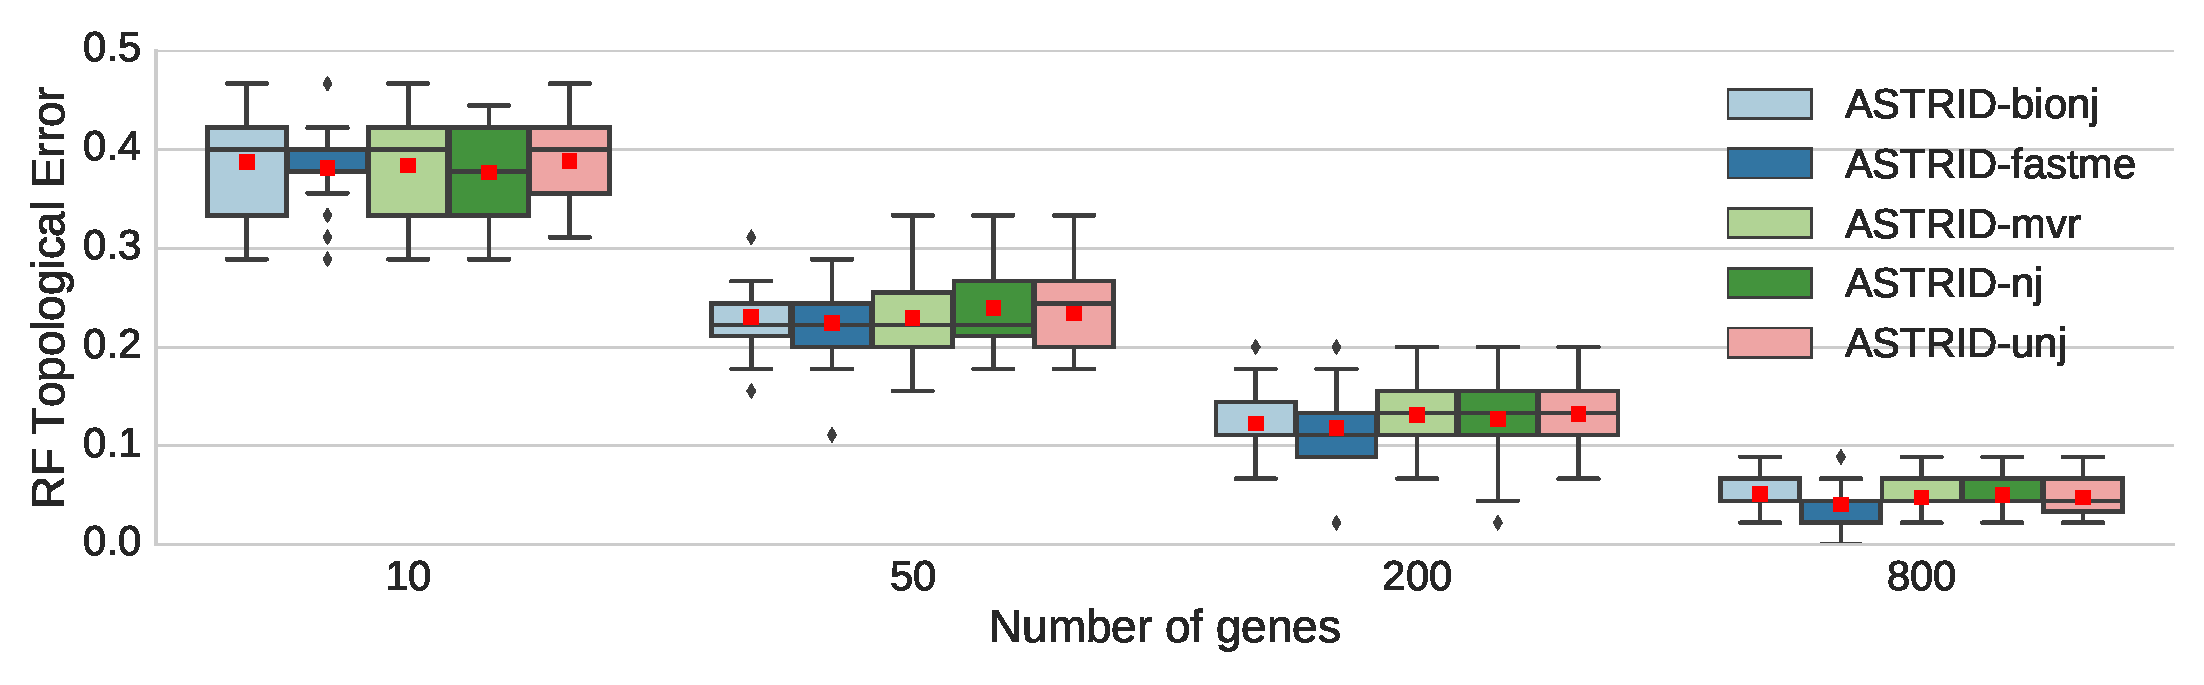
\includegraphics[width=12cm]{astrid-figs/avian-njcomparison.eps}
  \caption[Comparison of  ASTRID variants on
moderate ILS avian simulated datasets]{\textbf{A comparison of ASTRID variants on the
moderate ILS avian simulated datasets with 500bp, using 
different distance-based methods for the
      tree estimation phase.}
    We report RF topological error rates over 20 replicates. Red dots
    represent means, while lines represent medians and boxes represent
    quartiles. 
}
  \label{astrid::fig:avian-njcomparison}
\end{figure}


\begin{figure}
  \centering
  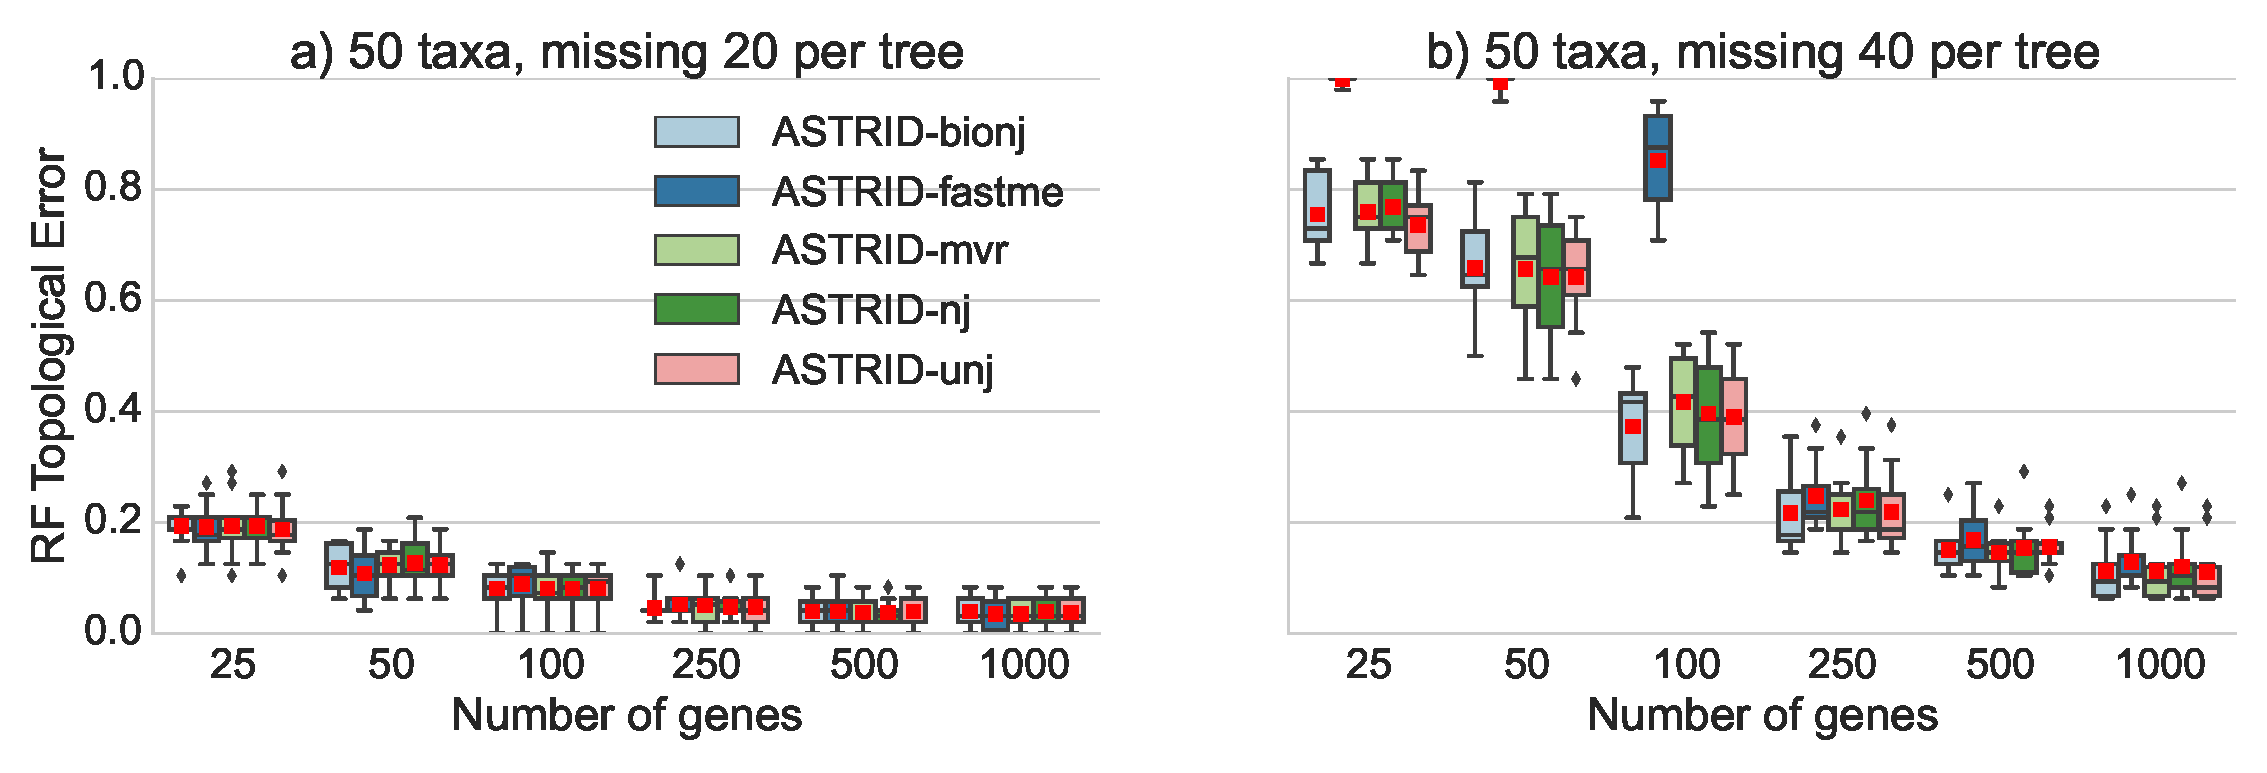
\includegraphics[width=12cm]{astrid-figs/astral2-missing-l300-njcomparison-main.eps}
  \caption[Comparison of ASTRID variants
on 50-taxon datasets with missing taxa.]{\textbf{Comparison of ASTRID variants
on 50-taxon ASTRAL-2 MC8 datasets with missing taxa.}
 We show
average RF error rates over 50 replicates for
ASTRID variants, that differ in terms of the method used
to compute the tree from the distance matrix. 
The datasets have  taxa randomly removed
    from each gene and the sequence lengths truncated to 300bp. 
    Red dots
    represent means, while lines represent medians and boxes represent
    quartiles.}
  \label{astrid::fig:astral2-missing-njcomparison-main-l300}
\end{figure}


\subsection{Comparison of ASTRID, ASTRAL, and MP-EST}


We begin with a comparison between ASTRID, ASTRAL-2, and MP-EST 
on the avian simulated datasets with high (1X) ILS, varying number
of genes  and sequence alignment lengths, but where
all genes are complete; see Figure \ref{astrid::fig:avian-mpest}.

\begin{figure}
  \centering
  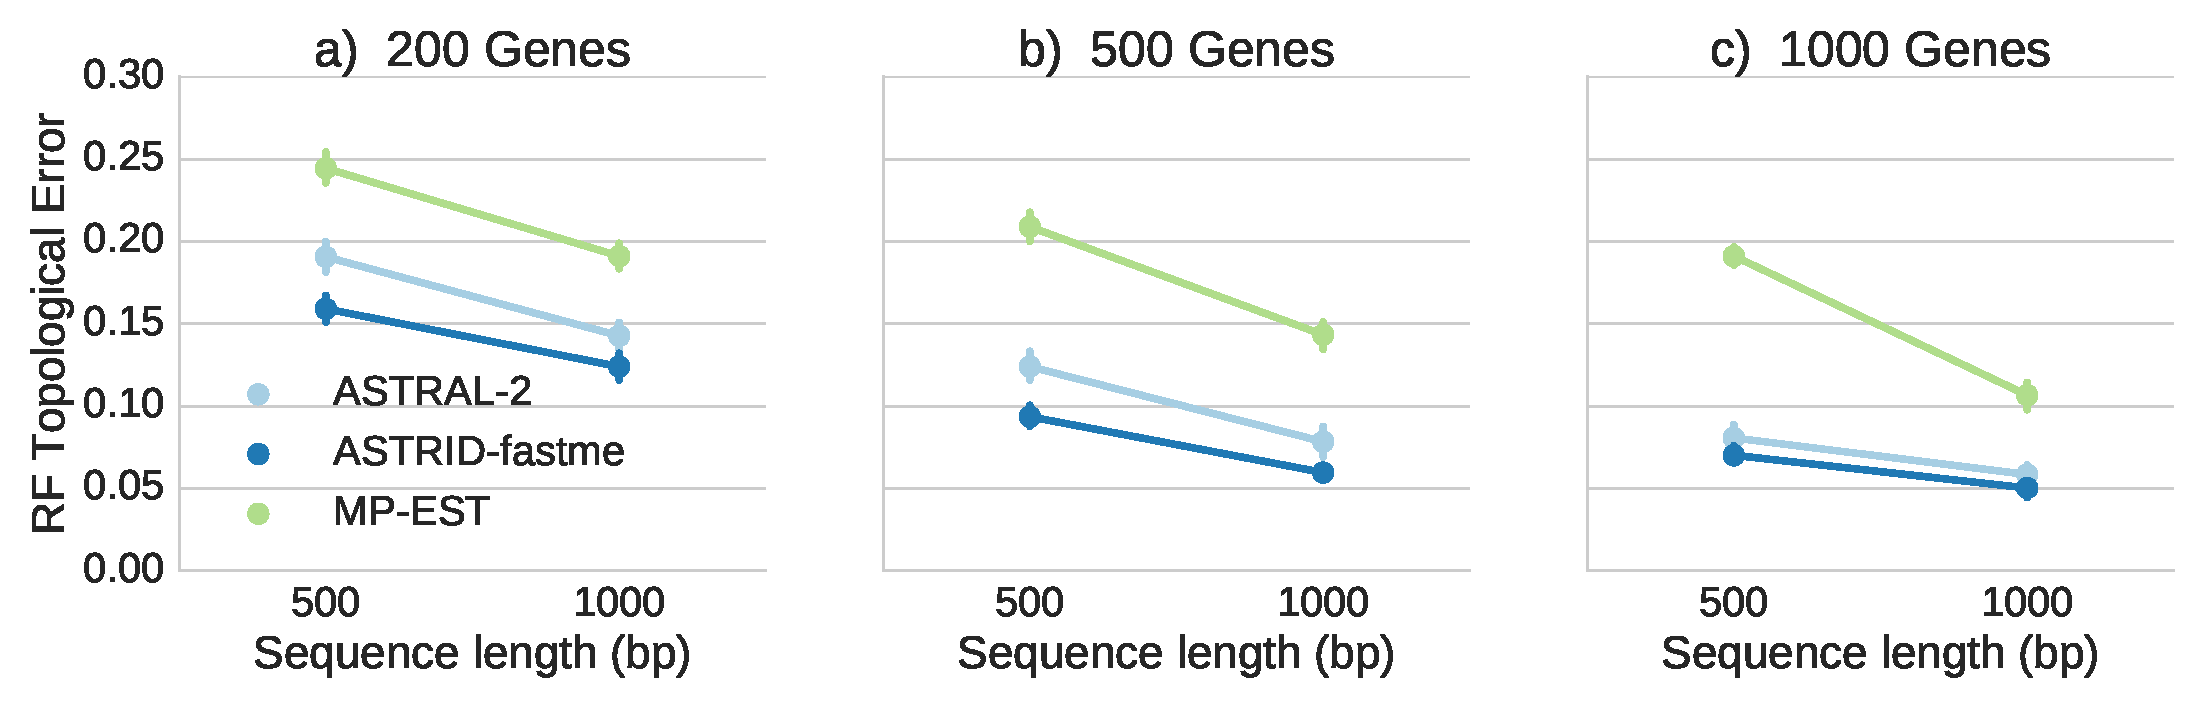
\includegraphics[width=12cm]{astrid-figs/avian-mpest.eps}
  \caption[Comparison of ASTRID, ASTRAL-2, and MP-EST 
      on avian simulated data]{\textbf{Comparison of ASTRID, ASTRAL-2, and MP-EST 
      on the avian simulated data.} The
simulated data evolve under 1X (high ILS) species tree branch lengths,
and with
      varying gene sequence lengths.
      We report mean RF rates with standard error bars over 20
    replicates. 
}
  \label{astrid::fig:avian-mpest}
\end{figure}
All methods improved with increasing numbers of genes
or increasing sequence length; however, the methods
differed substantially in terms of their accuracy.
Across all conditions we explored,
MP-EST had the highest error 
and ASTRID had the lowest  error. 
ASTRAL-2 was in between, but was closer to ASTRID than to 
MP-EST. 
The gap between MP-EST and ASTRID was very large,
and increased with the number of genes. For example,
at 1000 genes and gene sequence alignments of length 500,
MP-EST had 19\% RF error while
ASTRID had about 7\% RF error.
The gap between ASTRID and ASTRAL-2 was substantial 
on the 200- and 500-gene cases, but very small
on the 1000-gene case. 

Thus, although MP-EST is statistically consistent
under the MSC model
and hence theoretically robust to ILS, it 
did not have particularly good accuracy on
these data. 
Among all coalescent-based methods, 
MP-EST is probably the one that has been used the
most in biological data analyses, but
its performance here and
in \cite{ASTRALII,BayzidRECOMBCG2014} demonstrates that it is not
competitive with the best methods on  datasets
with even moderate numbers
of species. 
Therefore, we omit MP-EST from the rest of
this study.




\subsection{Comparison of ASTRID and ASTRAL-2 
on complete gene trees}

\paragraph{Comparison on avian datasets. }
Figure \ref{astrid::fig:avian-ils} shows the performance of
ASTRAL-2 
 and ASTRID on avian simulated datasets
under three ILS conditions (moderate, high, and very high).
Both methods performed better when provided with more genes, and both
performed worse on higher levels of ILS.
Overall, ASTRID tended to outperform ASTRAL-2, with the
largest effect seen when many genes were available. With 800 genes
available, the ASTRID species tree had a RF error
rate that was 2.4 percentage points better than ASTRAL-2’s under the
very high and high ILS model conditions, and 1.2 percentage points better for
the moderate ILS model condition.
On the moderate ILS model condition, ASTRID had the greatest advantage
over ASTRAL-2 
 for moderate numbers of genes. Above 200 genes, the error
rate dropped below ten percent for both ASTRAL-2 
 and ASTRID, and ASTRID
had an average advantage of only about one percentage point.


\begin{figure}
  \centering
  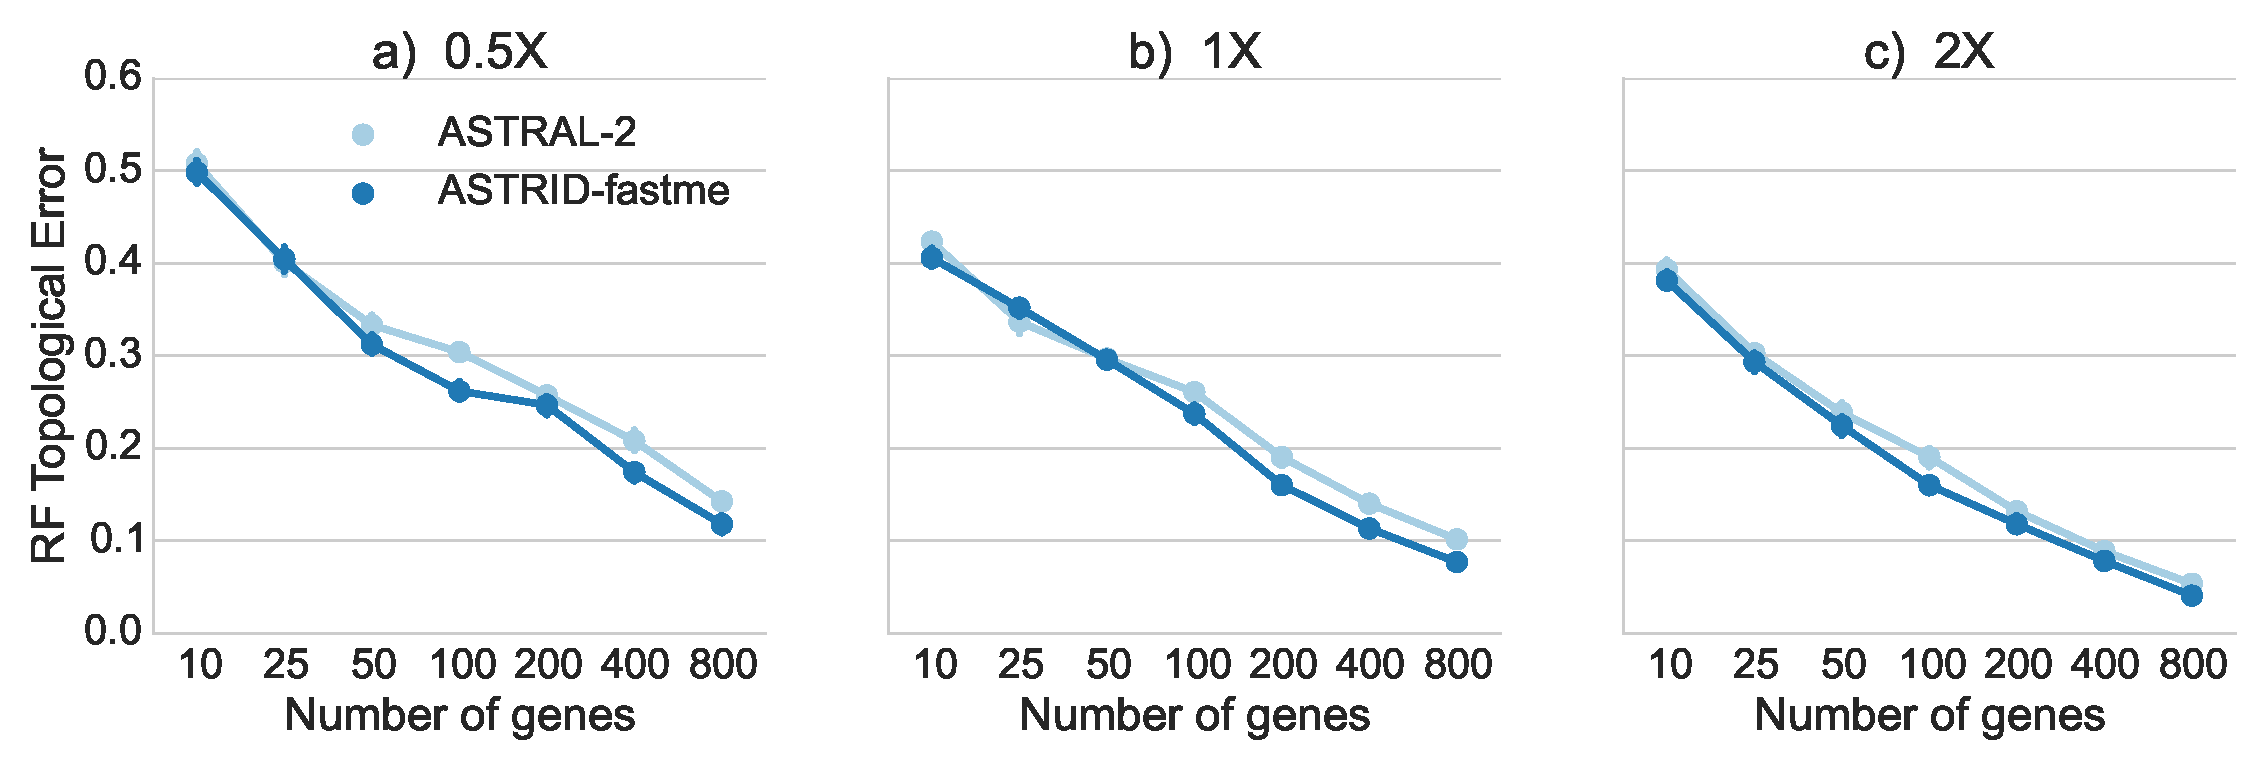
\includegraphics[width=12cm]{astrid-figs/avian-ils.eps}
  \caption[Comparison of ASTRID and ASTRAL-2 on avian simulated datasets]{\textbf{Comparison of ASTRID and ASTRAL-2 on avian simulated datasets. }
We show average RF error rates and standard error
bars for 20 replicates. Gene sequence alignments  have 500 sites
and
    varying amount of ILS. 
Species tree branch lengths of 0.5x 
    have very high ILS, 1X has high ILS, and 2x have moderate ILS. 
}
  \label{astrid::fig:avian-ils}
\end{figure}


It is well known that summary methods improve in accuracy as the
number of sites per gene or the number of genes increase
\cite{mirarab2014evaluating,GatesyMPE2014,bayzid2013naive,roch2015robustness}.  We
explored the impact of varying the sequence length and number of genes
on the avian datasets with high (1X) ILS, as well as on true gene
trees.  Figure \ref{astrid::fig:avian-seqlength} shows results on 10, 100, and
1000 genes; results on other numbers of genes have the same trends
(data provided in supplementary materials).
As expected, both methods improved
with increased sequence length, and had their best accuracy on
true gene trees.
Both methods also improved as the number of genes increased. 
ASTRID
was always at least as accurate as ASTRAL-2,
with the biggest improvement for shortest
sequences (with 250bp). 
 

\begin{figure}
  \centering
  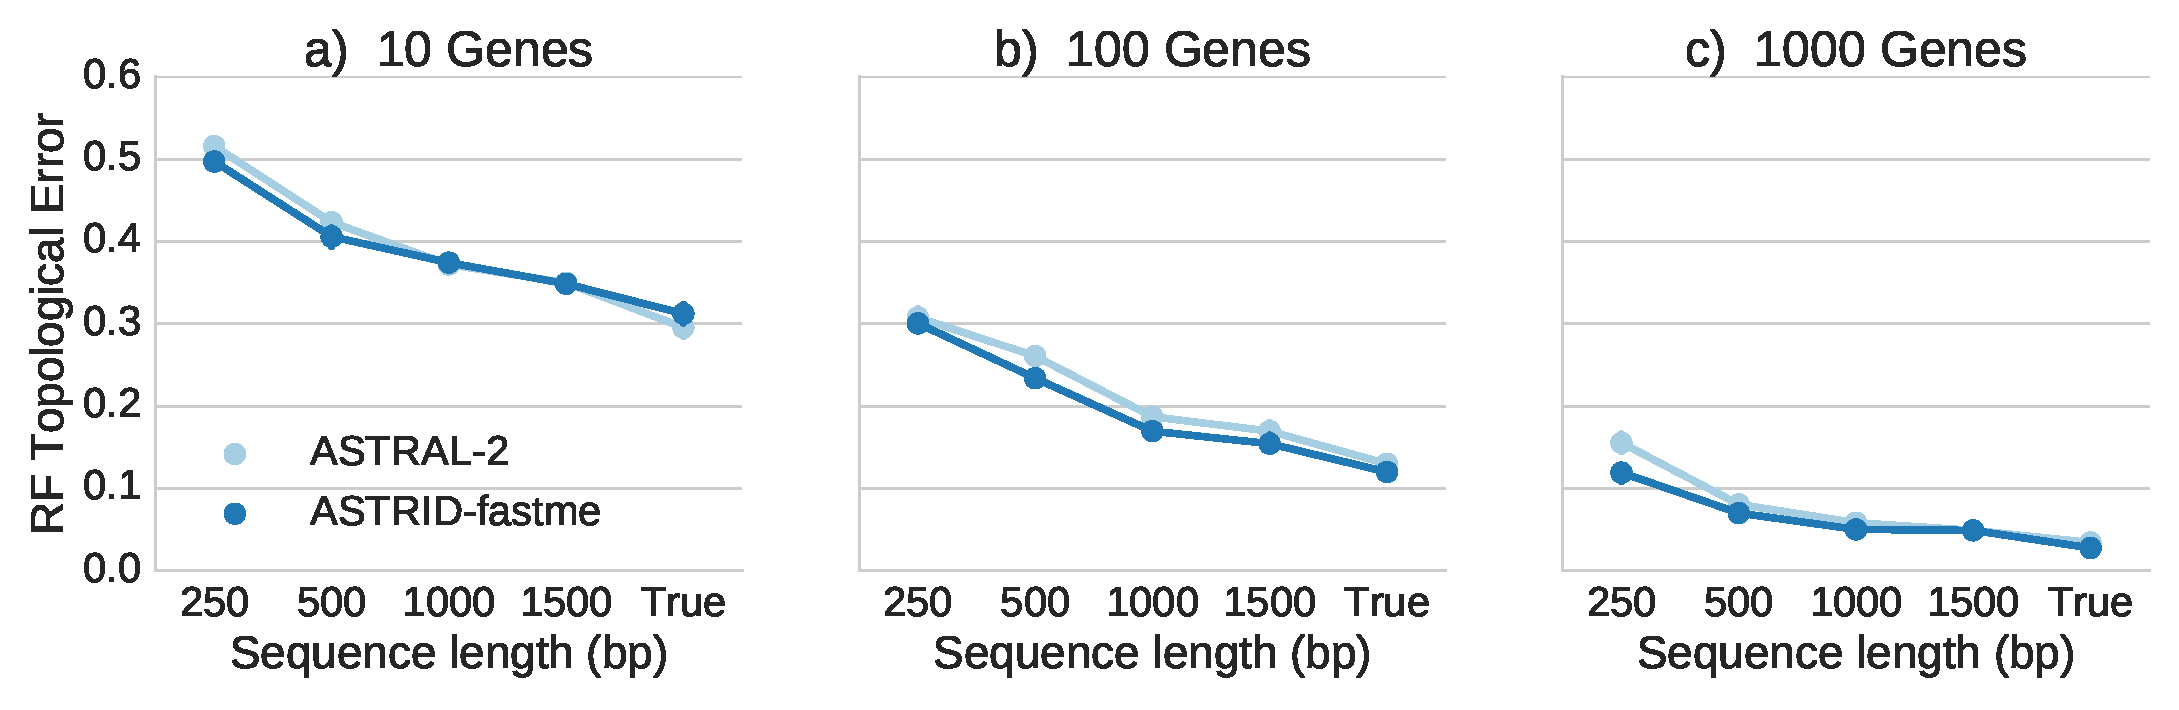
\includegraphics[width=12cm]{astrid-figs/avian-seqlength-main.eps}
  \caption[Performance on the avian simulated data with 1X
      species tree branch lengths]{\textbf{Performance on the avian simulated data with 1X
      species tree branch lengths, varying gene sequence length and
      number of genes.} We report RF  rates over 20
    replicates.}
  \label{astrid::fig:avian-seqlength}
\end{figure}

\paragraph{Comparison on mammalian datasets. }
A comparison of ASTRAL-2 
 and ASTRID on the mammalian datasets
with different levels of ILS (high, moderate, and low)
is given in 
Figure \ref{astrid::fig:mammalian-ils}.
ASTRAL-2 
 and ASTRID performed
fairly similarly on the low (2X branch lengths) and moderate (1X branch
lengths) ILS conditions. Under the high ILS level (0.5X branch lengths), ASTRAL-2 
 was fairly consistently more accurate than ASTRID, with the largest
improvement on the 10-gene case.

\begin{figure}
  \centering
  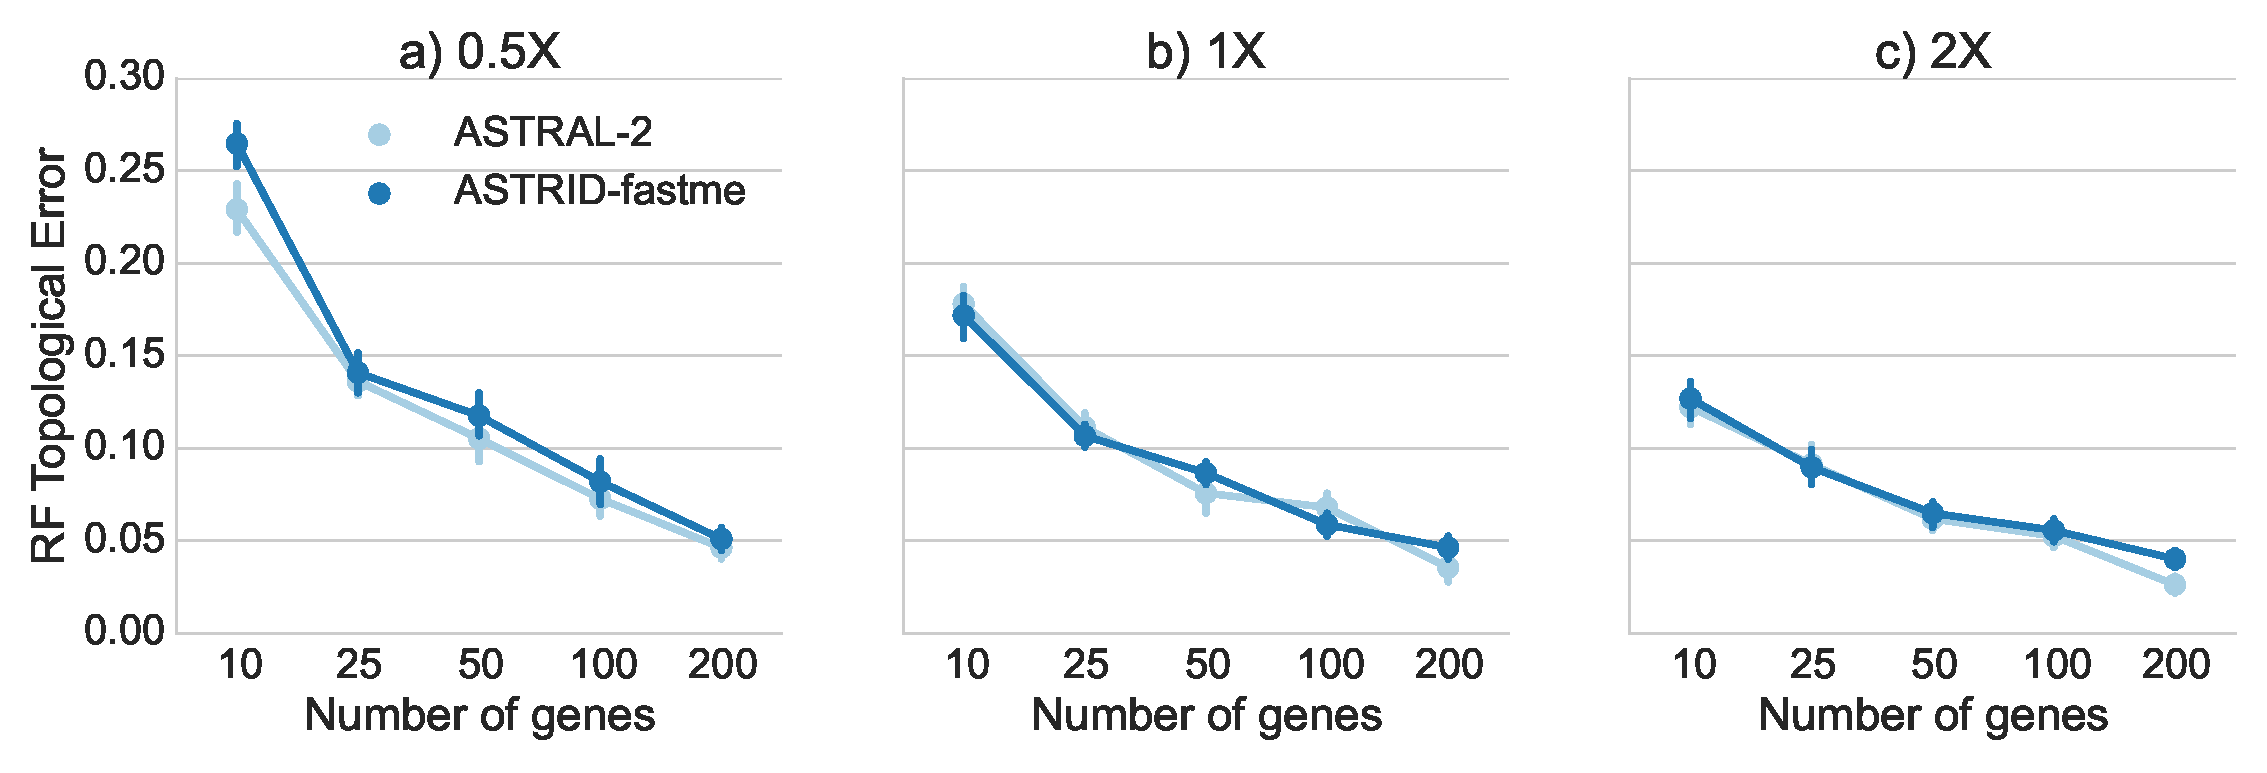
\includegraphics[width=12cm]{astrid-figs/mammalian-ils.eps}
  \caption[Comparison of methods on mammalian simulated datasets, varying ILS level and number of genes]{\textbf{Comparison of methods on mammalian simulated datasets, varying ILS level and number of genes.}  We
show average RF error rates and standard error bars for 20 replicates. 
Gene sequence alignments had
    500 sites. Model conditions varied in ILS level
from high (0.5x branch lengths) to low (2X branch lengths).
}
  \label{astrid::fig:mammalian-ils}
\end{figure}

\paragraph{Comparison on the ASTRAL-2 datasets. }
We explored performance on the ASTRAL-2 datasets
with 200 taxa (model conditions MC1 to MC6, see
Fig.~\ref{astrid::fig:astral2-ils}). % (i.e., MC1-MC6).
These model trees varied in ILS level, with MC1 and MC4 having 
very high ILS, MC2 and MC5 having moderate ILS, and
MC3 and MC6 having low ILS. 
Under MC2, MC3, and MC5, the two methods had 
essentially identical accuracy. However, under MC1, MC4, and MC6, 
ASTRAL-2 had an advantage over ASTRID.
In MC1 and MC4, the improvement disappeared at 100 genes,
but in MC6 ASTRAL-2 was still more accurate than ASTRID on 100 genes.


\begin{figure}
  \centering
  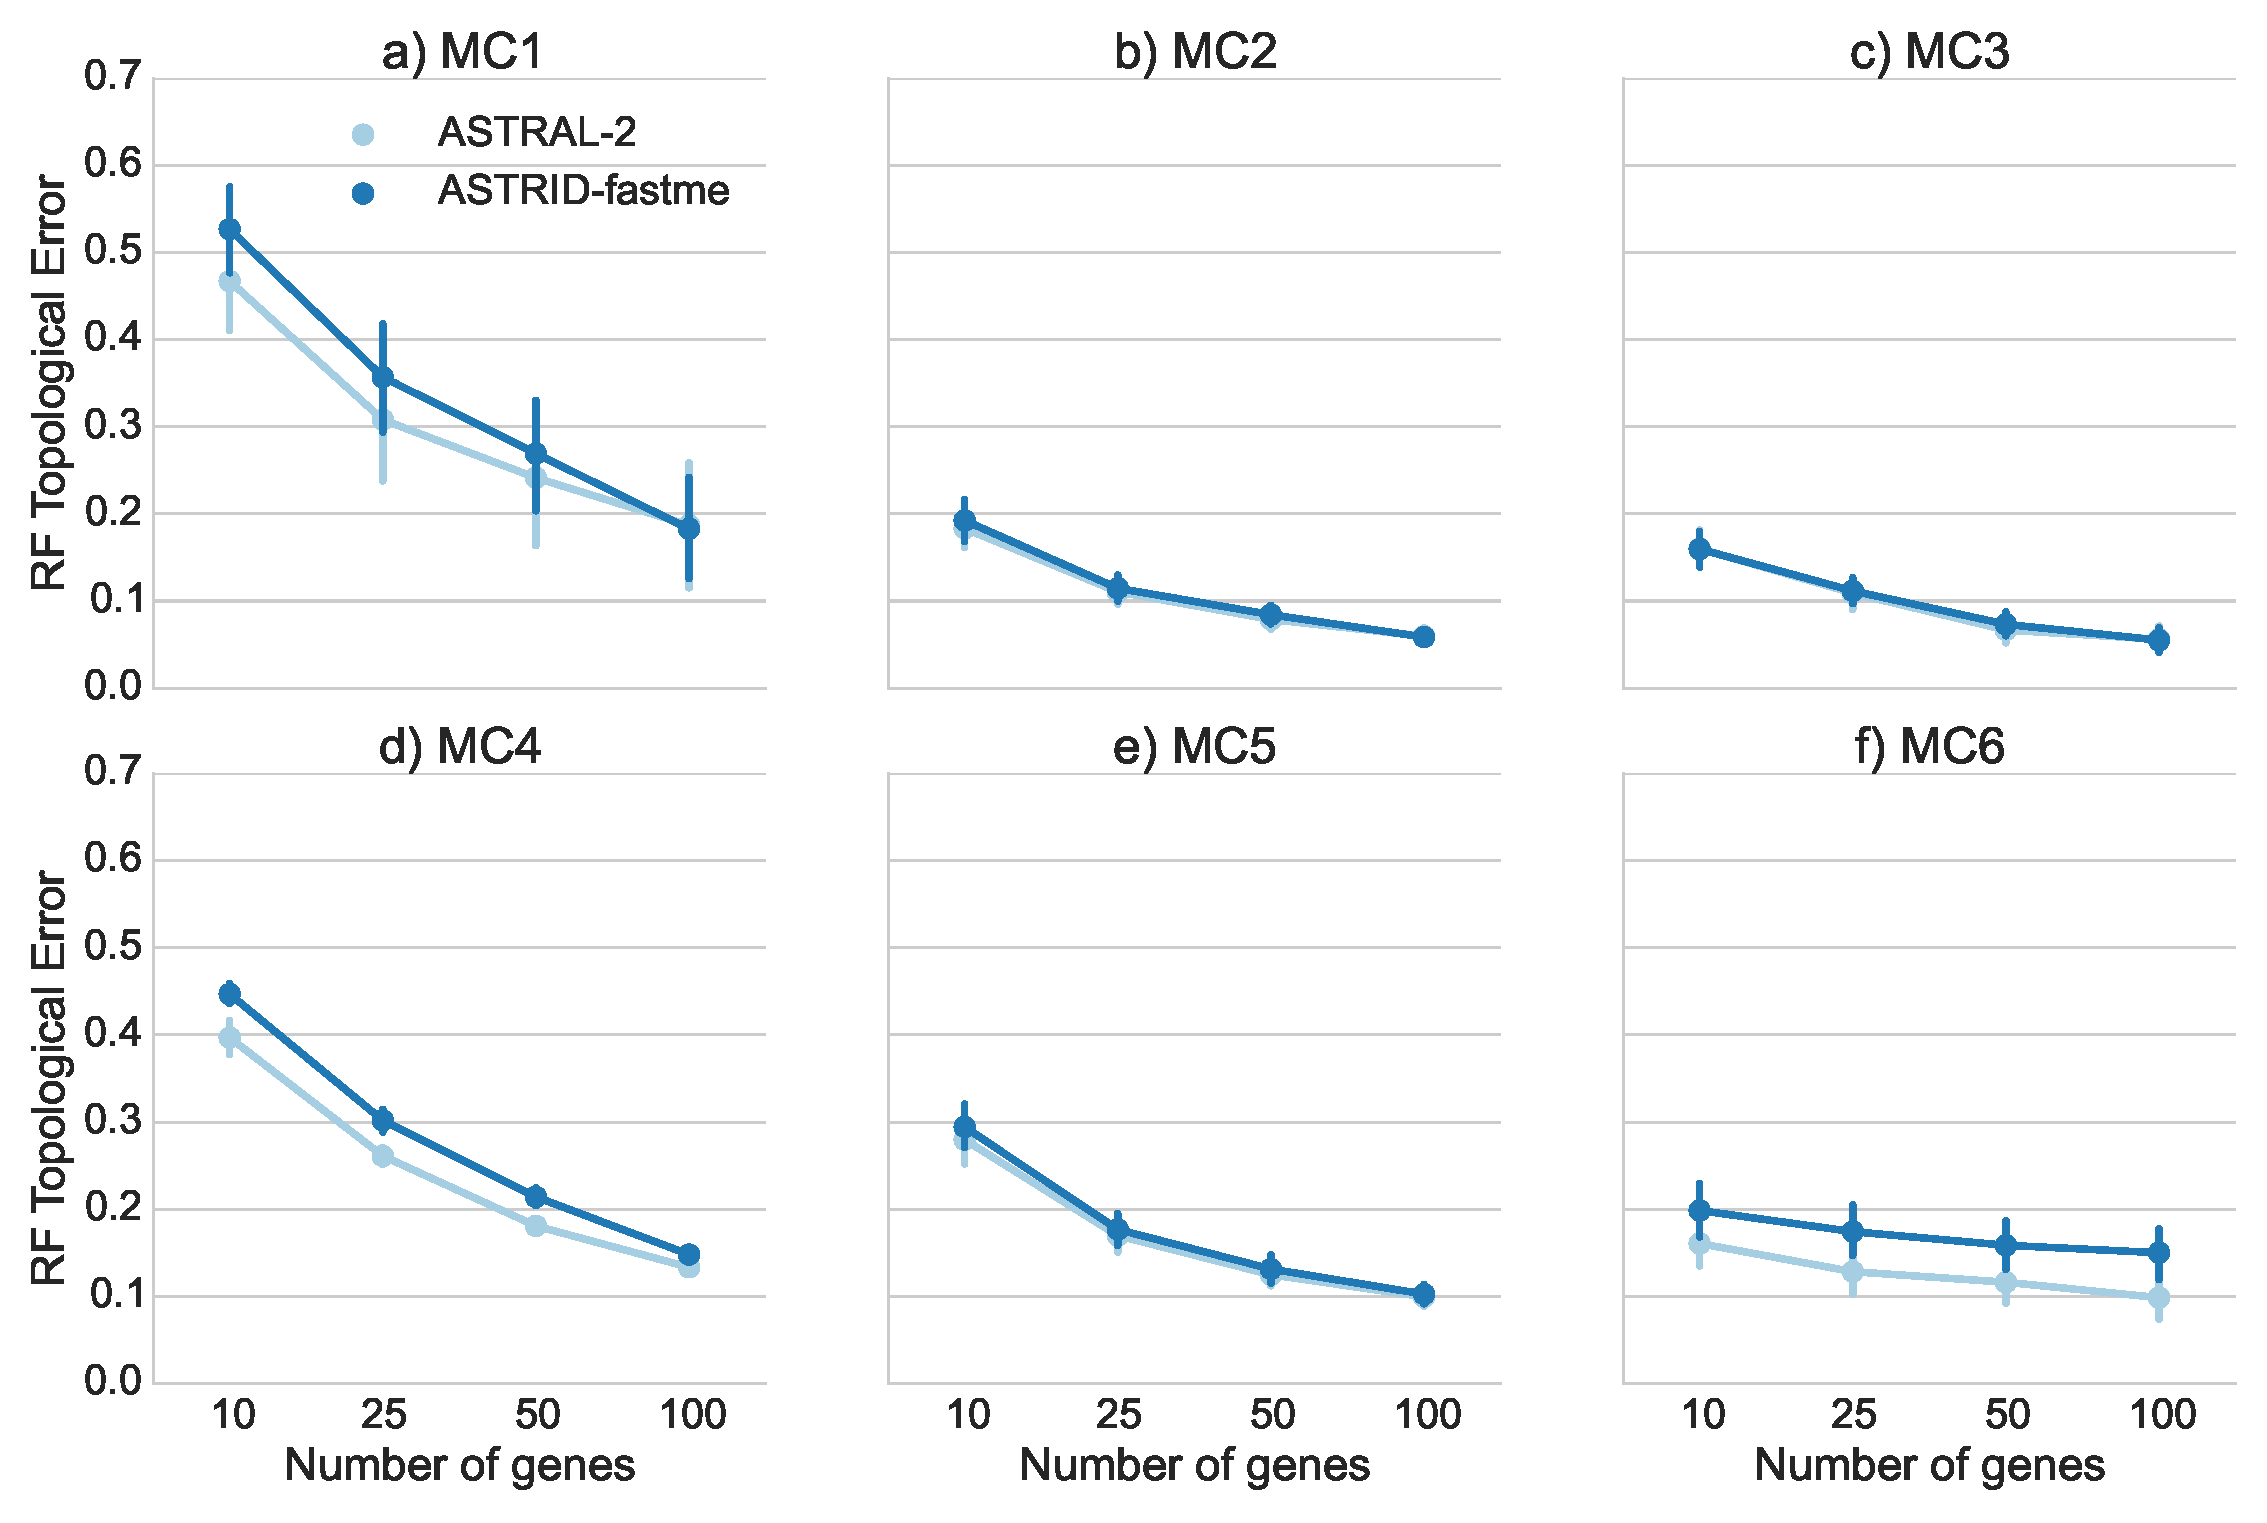
\includegraphics[width=12cm]{astrid-figs/astral2-ils.eps}
  \caption[Comparison of ASTRID and ASTRAL-2
 on the simulated ASTRAL-2 datasets]{\textbf{Comparison of ASTRID and ASTRAL-2
 on the simulated ASTRAL-2 datasets
      with 200 taxa, varying levels of ILS, tree shape, and number of genes.}
    %Speciation events in the $1e-6$ model condition tended to occur
    %near the tips of the tree, and speciation events in the $1e-7$
    %model condition tended to occur near the root. Fewer generations
    %correspond to higher levels of ILS. 
     We report RF error
    rates and standard error 
bars over 10 replicates. See Table \ref{astrid::table:datasets} for
information on the model conditions listed. }
  \label{astrid::fig:astral2-ils}
\end{figure}

\paragraph{Comparison  on the 15-taxon datasets. }
%Tandy - check multiple-labels
The 15-taxon datasets evolved on a caterpillar
species tree under very high ILS (AD=82\%), the highest
ILS considered in this study.
We explored performance under two sequence lengths (100bp and 1000bp)
and varied the number of genes from 10 to 1000. 
Results on the 15-taxon datasets (Fig.~\ref{astrid::fig:15taxon})
showed very close performance between ASTRID and ASTRAL-2.
On the 100bp alignments and on 1000bp alignments with
at least 100 genes, the  two methods could not be distinguished.
However, on 1000bp alignments with at most 50 genes, ASTRAL-2
had an advantage over ASTRID.
\begin{figure}
  \centering
  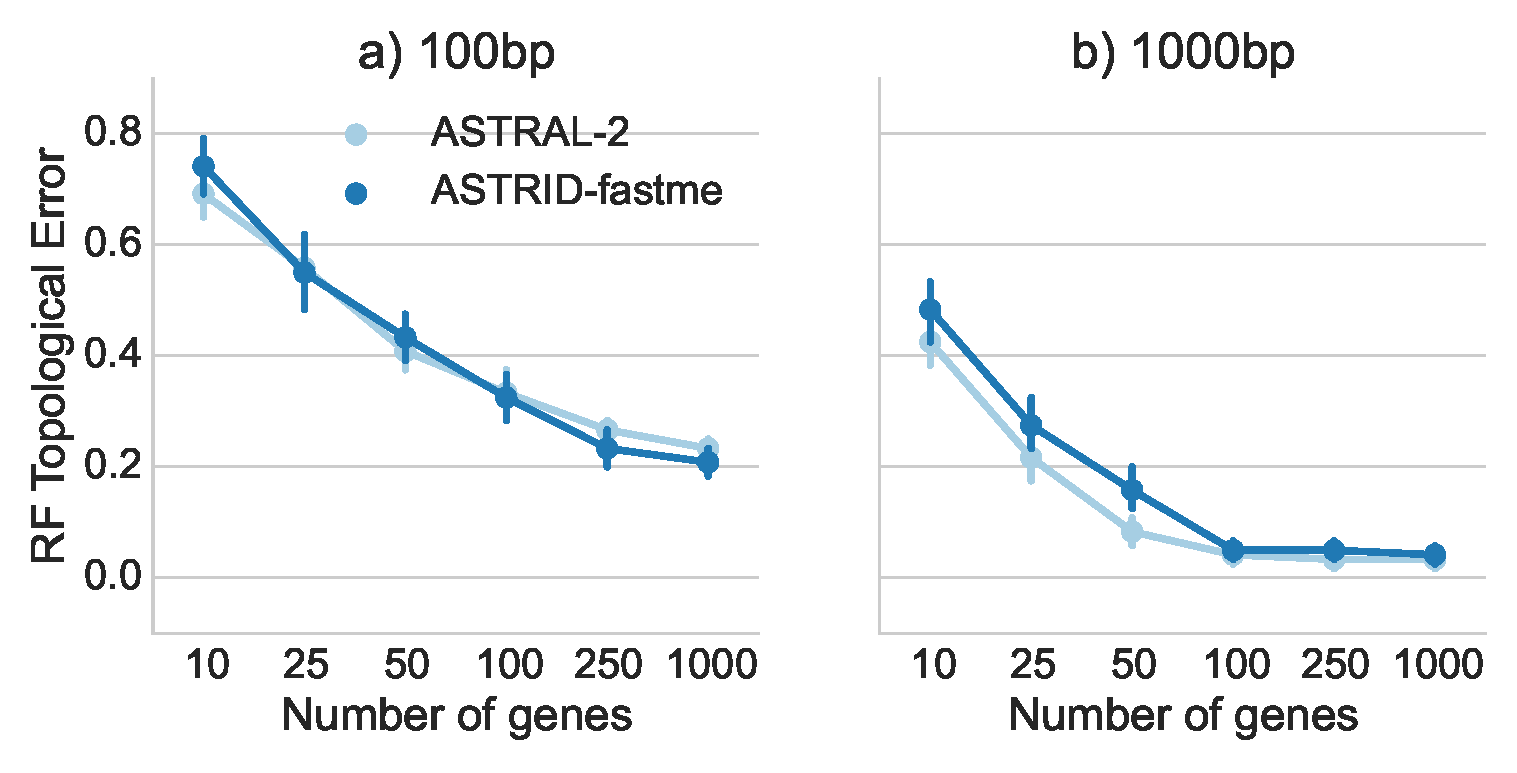
\includegraphics[width=12cm]{astrid-figs/15-taxon.eps}
  \caption[Comparison of ASTRID and ASTRAL-2  on the 15-taxon simulated
      datasets for two different sequence lengths]{\textbf{A comparison of ASTRID and ASTRAL-2  on the 15-taxon simulated
      datasets for two different sequence lengths.} The 15-taxon datasets
evolve down gene trees generated by a caterpillar
tree with very high ILS (AD=82\%), the highest ILS condition
explored in this study. We report mean RF 
      rates and standard error over 10 replicates. 
}  
  \label{astrid::fig:15taxon}
\end{figure}

\paragraph{Comparison on the 10-taxon datasets. }
The 10-taxon datasets evolved under two different ILS levels - high
and very high, and we explored performance  on both true and
estimated
gene trees; see Figure \ref{astrid::fig:10-taxon}.
In general, ASTRID and ASTRAL-2 had very close accuracy
on these data, but
there were some cases where they had different accuracy levels.
For example, on the high ILS condition with estimated
gene trees, ASTRAL-2 
 was more accurate 
than ASTRID for 200 genes, and ASTRID was
more accurate than ASTRAL-2 
 on 25 genes.





\begin{figure}
  \centering
  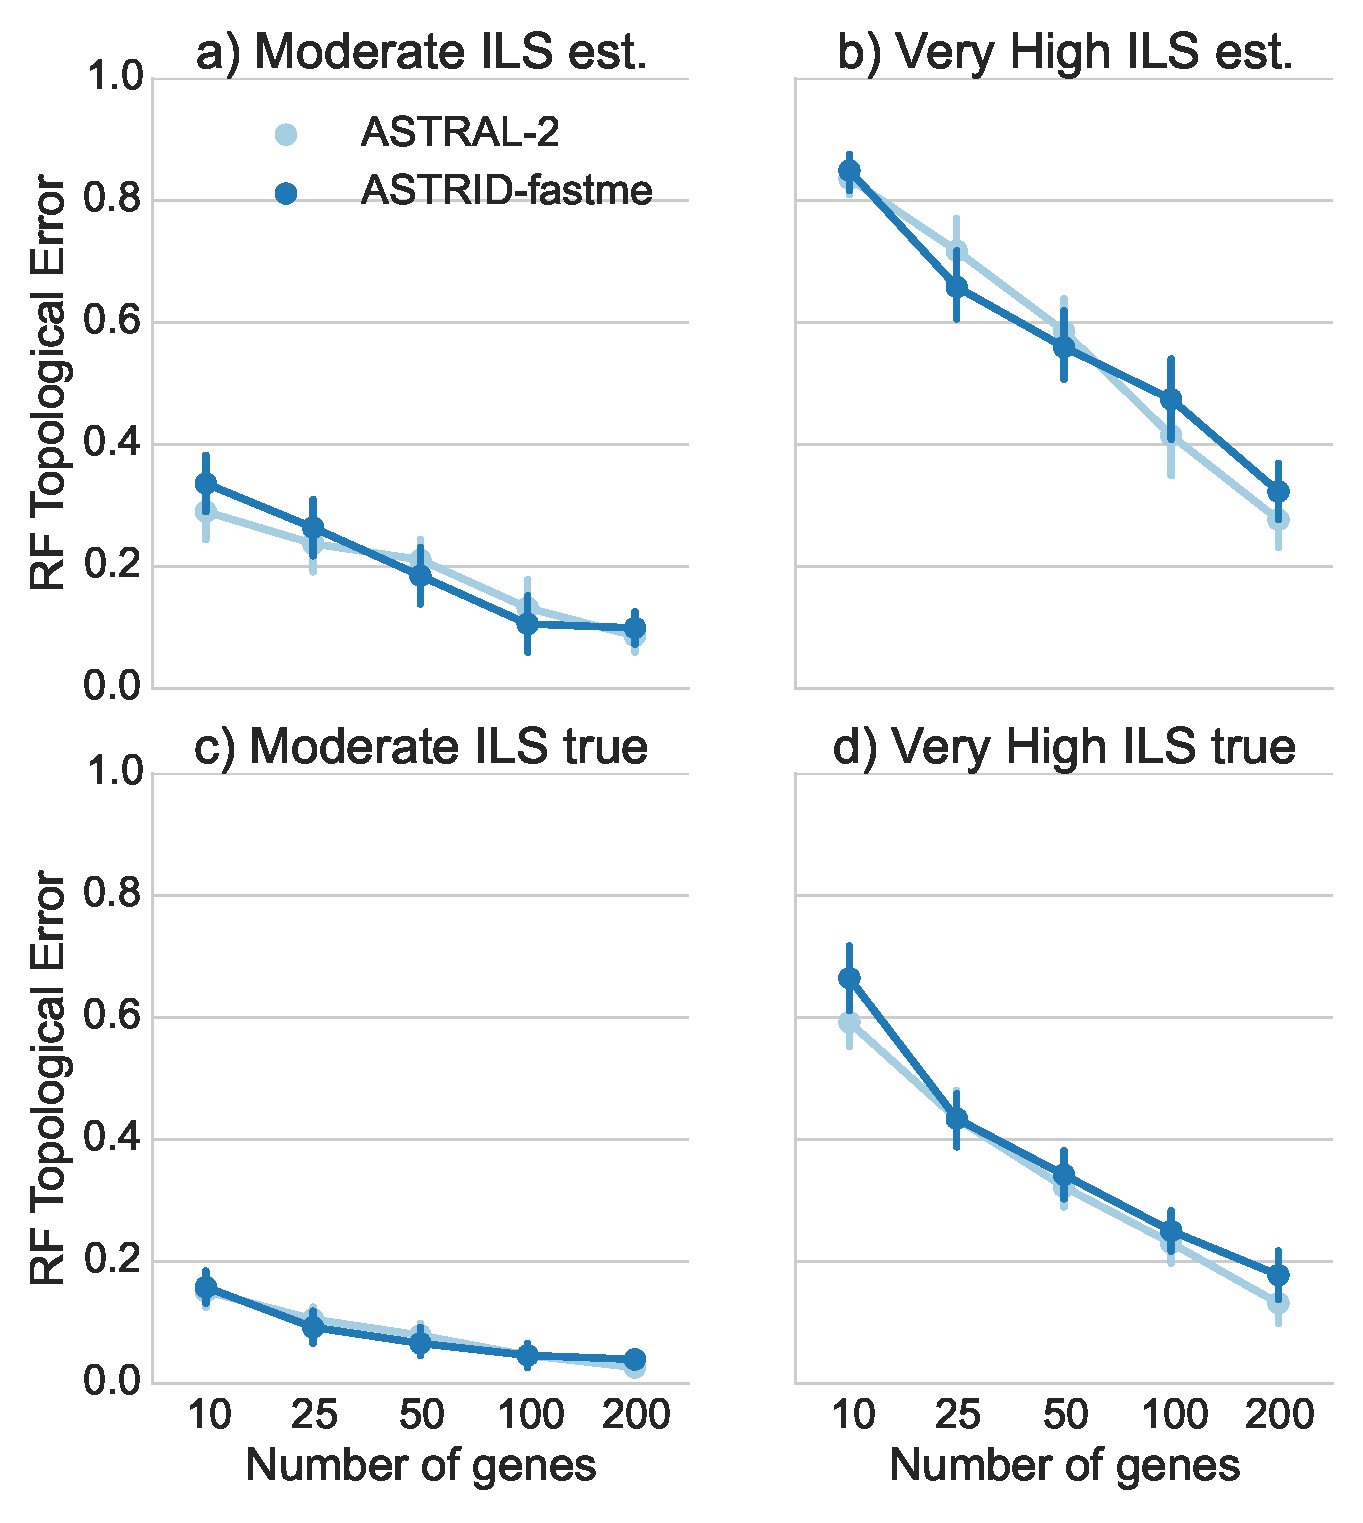
\includegraphics[width=12cm]{astrid-figs/10-taxon.eps}
  \caption[Results on true and estimated gene trees on 10-taxon datasets
with two ILS levels]{\textbf{Results on true and estimated gene trees on 10-taxon datasets
with two ILS levels (high and very high).}
      All gene sequence alignments have 100bp. We report RF rates and standard error bars over 20
    replicates. 
}
  \label{astrid::fig:10-taxon}
\end{figure}


\subsection{Performance on incomplete gene trees}
We explored the impact of missing data on
ASTRAL-2 and ASTRID by deleting taxa from gene trees
in the 
50-taxon datasets (MC8) from the ASTRAL-2 collection, 
using
150bp per gene, and varying the
number of genes and the amount of missing taxa; see Figure
\ref{astrid::fig:astral2-missing}. 
ASTRAL-2 
 and ASTRID had 
very similar 
topological accuracy throughout
these experiments. With low amounts of
missing data (20\% to 40\% missing taxa from each
gene tree), both methods had very good
accuracy (below 5\% tree error) by 500
genes. With 60\%  of the taxa missing from each gene tree,
the error rates increased for low
numbers of genes (above 20\% RF error for
up to 100 genes), but then declined to about 10\% by
1000 genes. 
With 80\% of the taxa missing from
each gene (so that all gene trees have only 10 taxa out of 50),
error rates were very high with 
25 genes (at least 85\% RF), but decreased quickly with increases
in the number of genes, so that
at 500 genes the error rate was 24\%, and
then at most 18\% at 1000 genes.
The trends suggest that
the error rates had not plateaued, and that adding additional
incomplete gene trees should result in continued improvement.

\begin{figure}
  \centering
  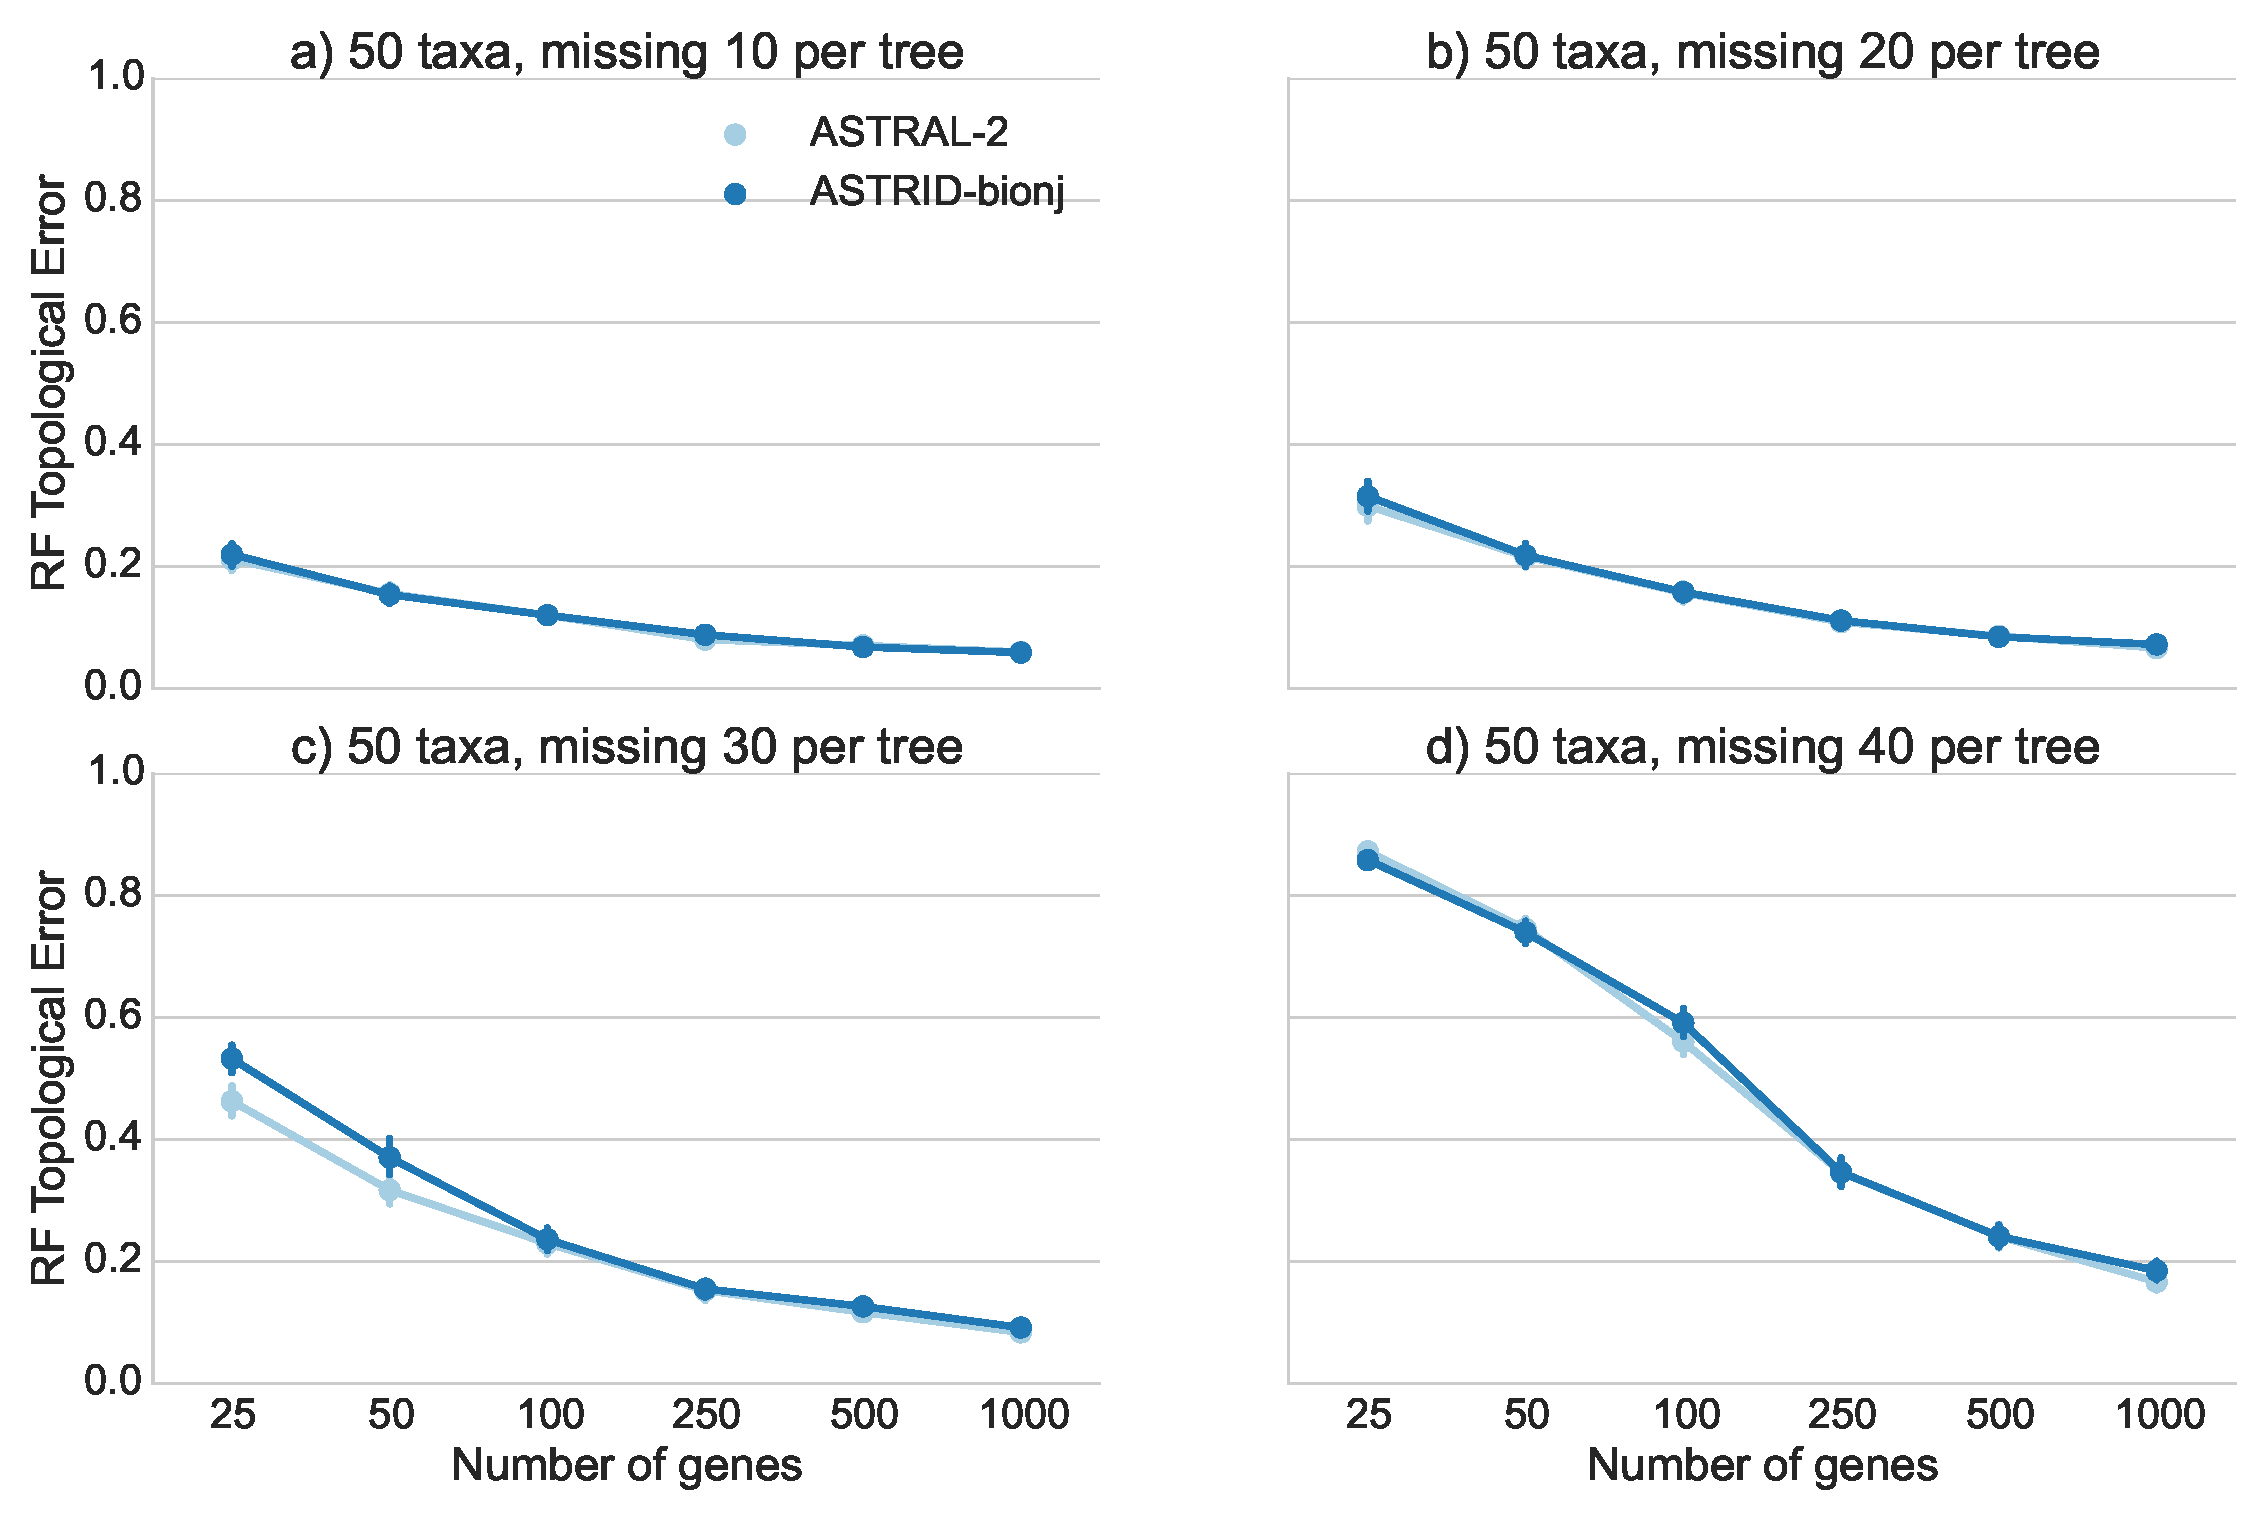
\includegraphics[width=12cm]{astrid-figs/astral2-missing.eps}
  \caption[Results on 50-taxon ASTRAL-2 dataset with
missing  taxa ]{\textbf{Results on 50-taxon ASTRAL-2 dataset (MC8) with
missing  taxa 
    and sequence lengths of 150bp.} We
    report RF rates and standard error over 50 replicates. 
}
  \label{astrid::fig:astral2-missing}
\end{figure}



\subsection{Analysis of the mammalian biological dataset}
We analyzed the mammalian biological dataset originally
studied in \cite{song2012}.  
The original
dataset had 37 species and 447 genes, but
there were 23
erroneous genes (as noted by \cite{statbinning}) which
we removed before doing the analysis. 

We obtained maximum likelihood gene trees and bootstrap
replicates of these gene trees from \cite{mirarab2014statistical}.
We then analyzed these
data using ASTRAL-2 and ASTRID+FastME
and compared these analyses to 
previously published trees obtained using ASTRAL
and MP-EST \cite{ASTRAL}. 
We then annotated the branches of the ASTRID+FastME and ASTRAL-2 trees with
bootstrap support from 100 multi-locus bootstrapping (MLBS).
The ASTRID+FastME and ASTRAL-2 trees
were topologically identical to the ASTRAL tree and differed
only in the bootstrap support;  
see Figure \ref{astrid::fig:astrid-biological} for the ASTRID+FastME tree.
On the other hand, the support for
the placement of Scandentia - one of the major
open questions about mammalian evolution - was very low,
only 47\% (ASTRAL-2 gave it 82\%). 
Hence, neither the ASTRID tree nor the ASTRAL-2 tree
resolved the placement of Scandentia
with high support.


\begin{figure}
\centering
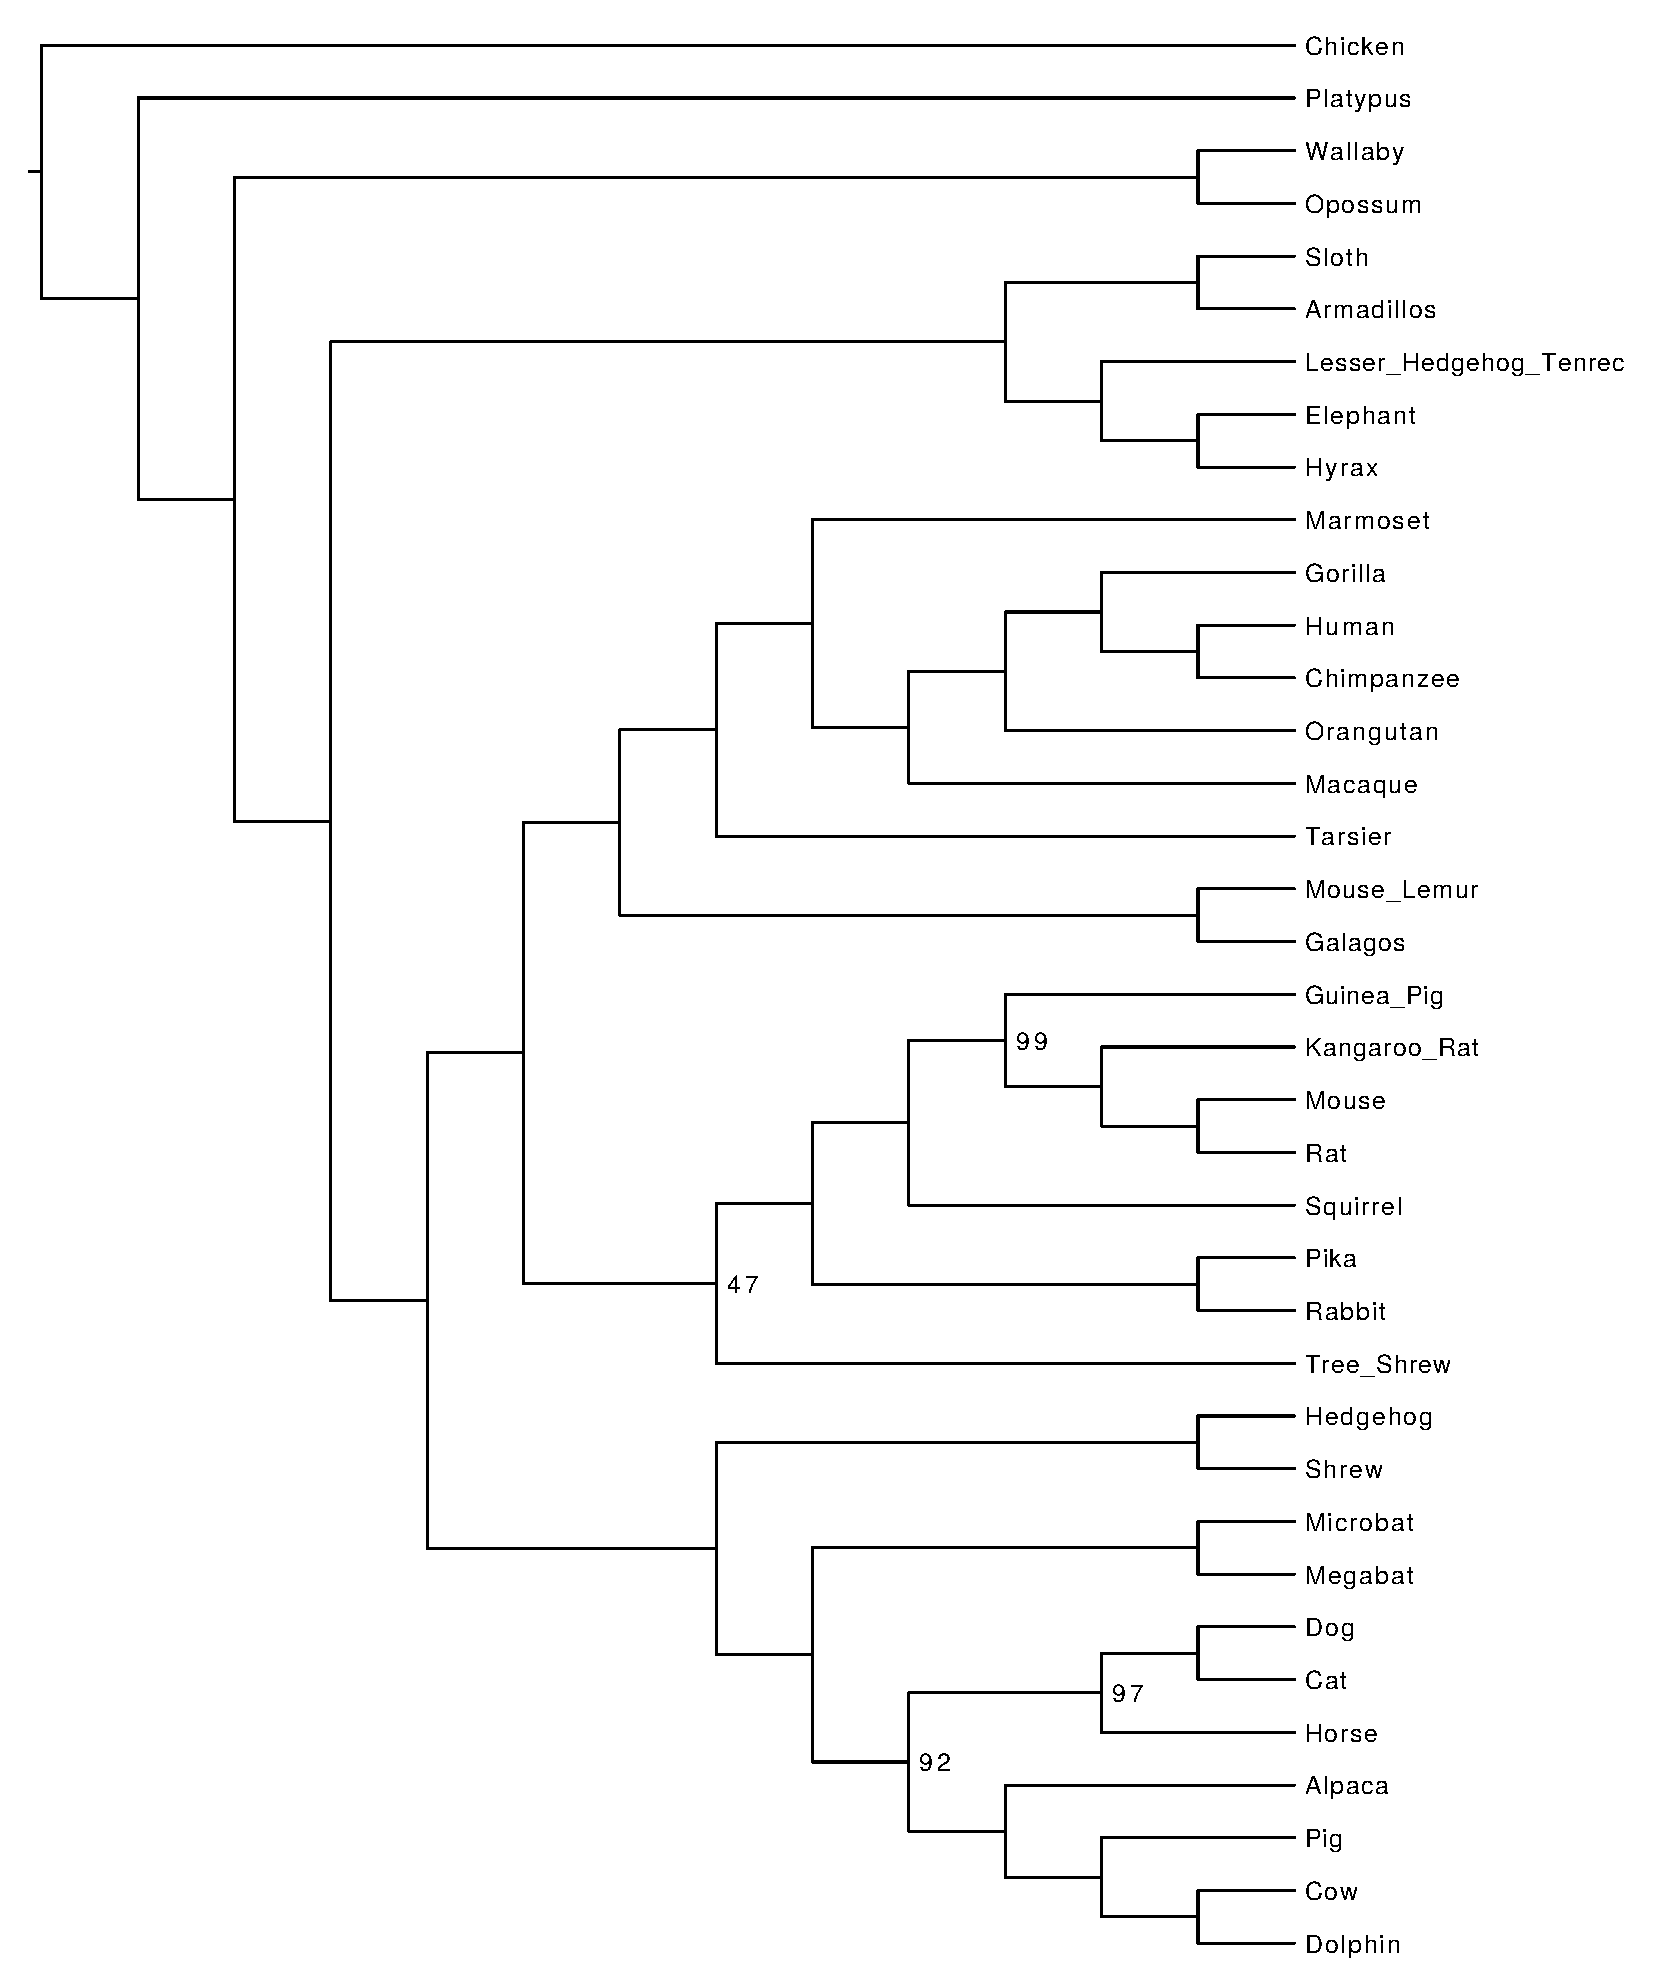
\includegraphics[width=12cm]{astrid-figs/astrid-biological.eps}
%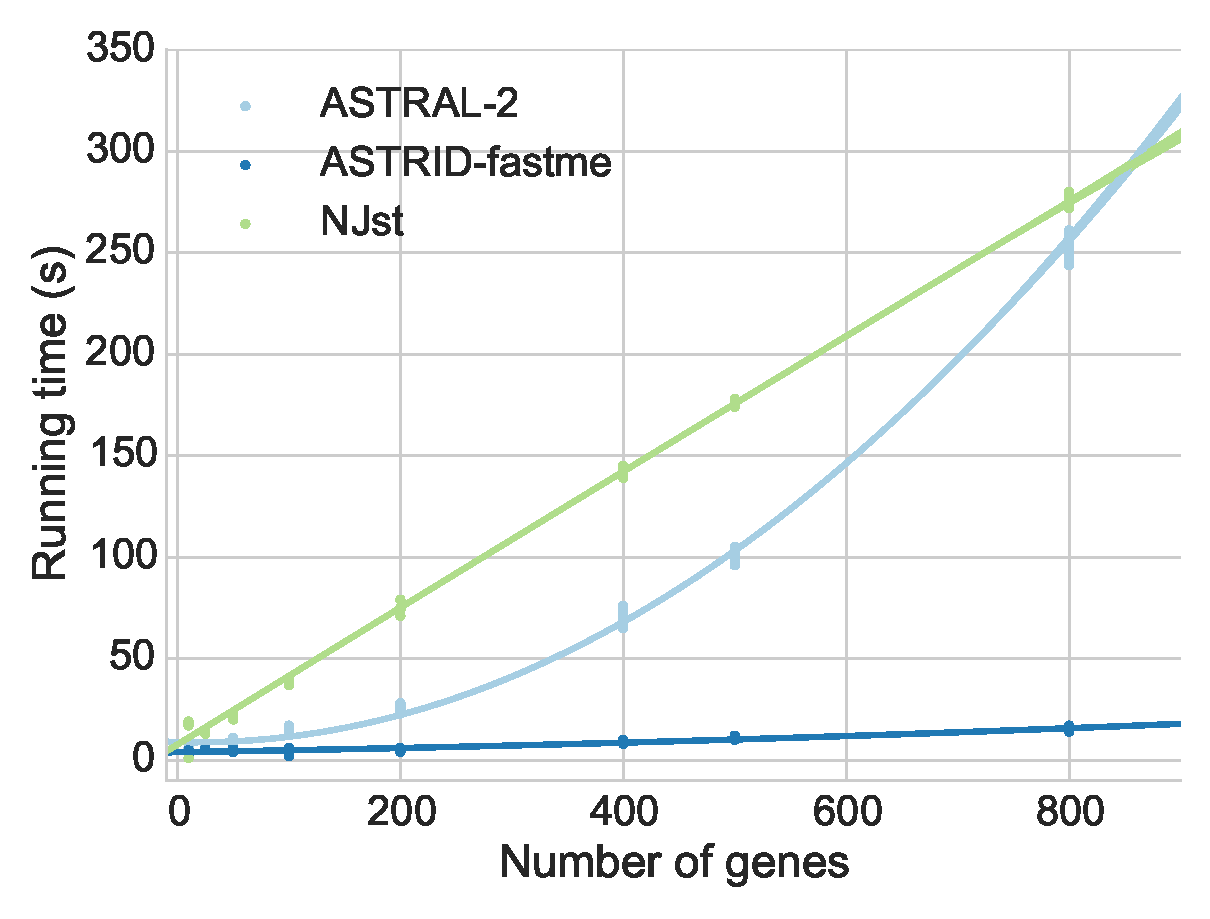
\includegraphics[width=12cm]{astrid-figs/avian-timing.eps}
  \caption[ASTRID analysis of a mammalian
biological dataset]{\textbf{ASTRID analysis of a mammalian
biological dataset.} 
We used ASTRID+FastME to 
analyze the mammalian biological dataset 
studied in \cite{statbinning,ASTRAL}, with 37 taxa and
424 genes. 
The branches are
annotated with 
bootstrap support values from 100 MLBS bootstrap samples;
values not shown indicate 100\% support.
The ASTRID tree is identical to the ASTRAL and ASTRAL-2 trees on the same data,
but differs from the MP-EST analysis in the placement of Scandentia.}
  \label{astrid::fig:astrid-biological}
\end{figure}




\subsection{Running time results}

\subsection{Asymptotic running time}

ASTRID has two steps: the first step computes the distance matrix, and
the second step uses a selected distance-based method to construct a
tree from the distance matrix.  When the input has $n$ species and $k$
genes, then calculating the distance matrix can be performed in
$O(kn^2)$ time.  Distance-based tree estimation methods typically run
in $O(n^2)$  to $O(n^3)$ time, but this step no longer depends on $k$.
Hence, the overall running time depends on the selected distance-based
method, but is generally dominated by the first phase, especially for
typical inputs, for which $k >> n$. Thus, under the assumption that
$k > n$ and that ASTRID uses a distance-based
method that runs in $O(n^3)$ time, ASTRID’s running time is $O(kn^2)$.

ASTRAL-2's scaling is more complicated to discuss.
Asymptotically, ASTRAL-2 runs in $O(n k |X|^2)$ time, where
$n$ is the number of species, $k$ is the number of genes, and $X$ is
a set of bipartitions it computes to constrain
the search space. The size of $X$ is not bounded by a polynomial
in the input size, and the technique that ASTRAL-2 uses
means that $X$ can be large under conditions with
high ILS. 
Thus the asymptotic running times of ASTRAL-2 and ASTRID (used with
various distance methods) are quite 
different. 

\subsection{Running times on simulated data}
In practice, creating the distance matrix took the majority of the
running time. On 1000 taxa, creating the distance matrix took several
minutes to several hours, depending on the number of genes, but
running $FASTME$ took less than one second regardless of the number of
genes. However,  PhyD* methods were much
slower than $FASTME$; on 1000 taxa, running any of the PhyD* methods
took approximately 40 minutes (data not shown).




We recorded running
times for ASTRAL-2, 
ASTRID-FastME, and NJst, 
on avian 
simulated datasets with high ILS (1X),
as
we varied the number of genes (see Fig.~\ref{astrid::fig:avian-timing}).
Note that ASTRID-FastME was by far the fastest of the three
methods, and NJst was the slowest. However, the trends suggest
that NJst will be faster than ASTRAL-2 for larger numbers of genes.
Note also that ASTRID-FastME and NJst both scaled linearly with the
number of genes, but that ASTRAL-2’s running time scaled super-linearly.

We recorded running times for two variants of ASTRID
(one using FastME and the other using BioNJ*), and compared them
to ASTRAL-2 on ASTRAL-2 simulated datasets  with
1000 taxa (MC11) as we varied the number of genes
(Fig.~\ref{astrid::fig:1000-timing}) and for 500-gene datasets
in which we varied the number of taxa (MC 2 and 7-10, see Fig.~\ref{astrid::fig:astral-timing}).
The relative running times show that all methods were
very fast for smaller datasets, but were clearly distinguished
on the larger datasets, where 
ASTRID-FastME was much faster than ASTRID-BioNJ* and 
both variants of 
ASTRID were much faster than ASTRAL-2.  
For example, on the dataset with 1000
genes and 1000 taxa, ASTRID-FastME
finished in 33 minutes, ASTRID-BioNJ finished in 1 hour and 10
minutes, and ASTRAL-2 finished in 12 hours and 30 minutes.


\subsection{Running times on biological data}
We recorded running times for ASTRID-FastME and ASTRAL-2 on the
mammalian biological dataset. Both methods took 6 seconds for a
single bootstrap replicate on one core of a 2.7 GHz Intel Xeon
processor with 424 genes and 37 taxa. 
 
\begin{figure}
  \centering
  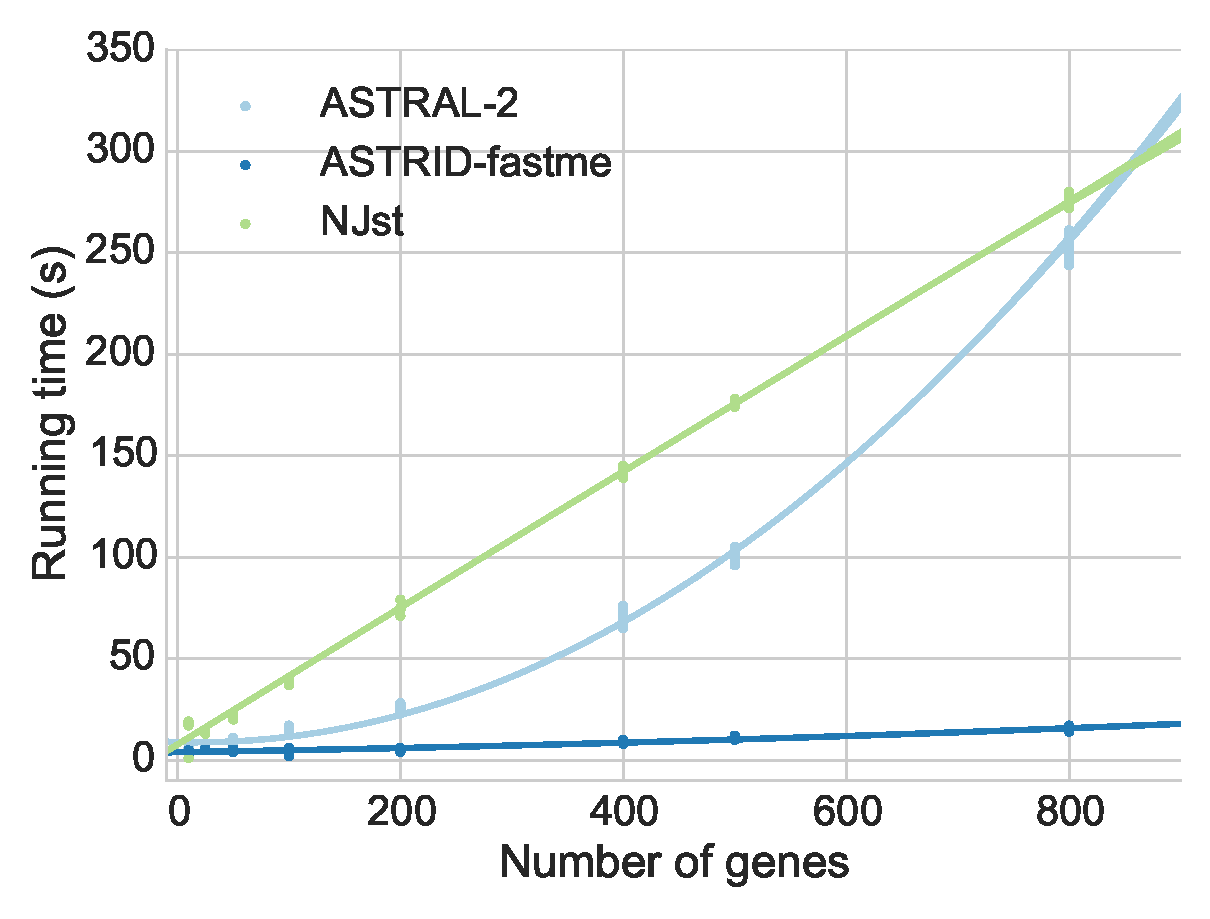
\includegraphics[width=12cm]{astrid-figs/avian-timing.eps}
  \caption[Running times for
ASTRID-FastME, ASTRAL-2, and NJst,  on avian high ILS
(1X) simulated datasets]{\textbf{Scatterplot of running times for
ASTRID-FastME, ASTRAL-2, and NJst,  on avian high ILS
(1X) simulated datasets, varying number
    of genes.} We show running time for 20 replicates of each
number of genes.    The quadratic dependence of ASTRAL-2's 
 running time is
    clearly contrasted with the linear
dependence of both ASTRID and NJst. 
    Experiments were run on a single core of a
    2.7 GHz Intel Xeon processor.}
  \label{astrid::fig:avian-timing}
\end{figure}


\begin{figure}
  \centering
  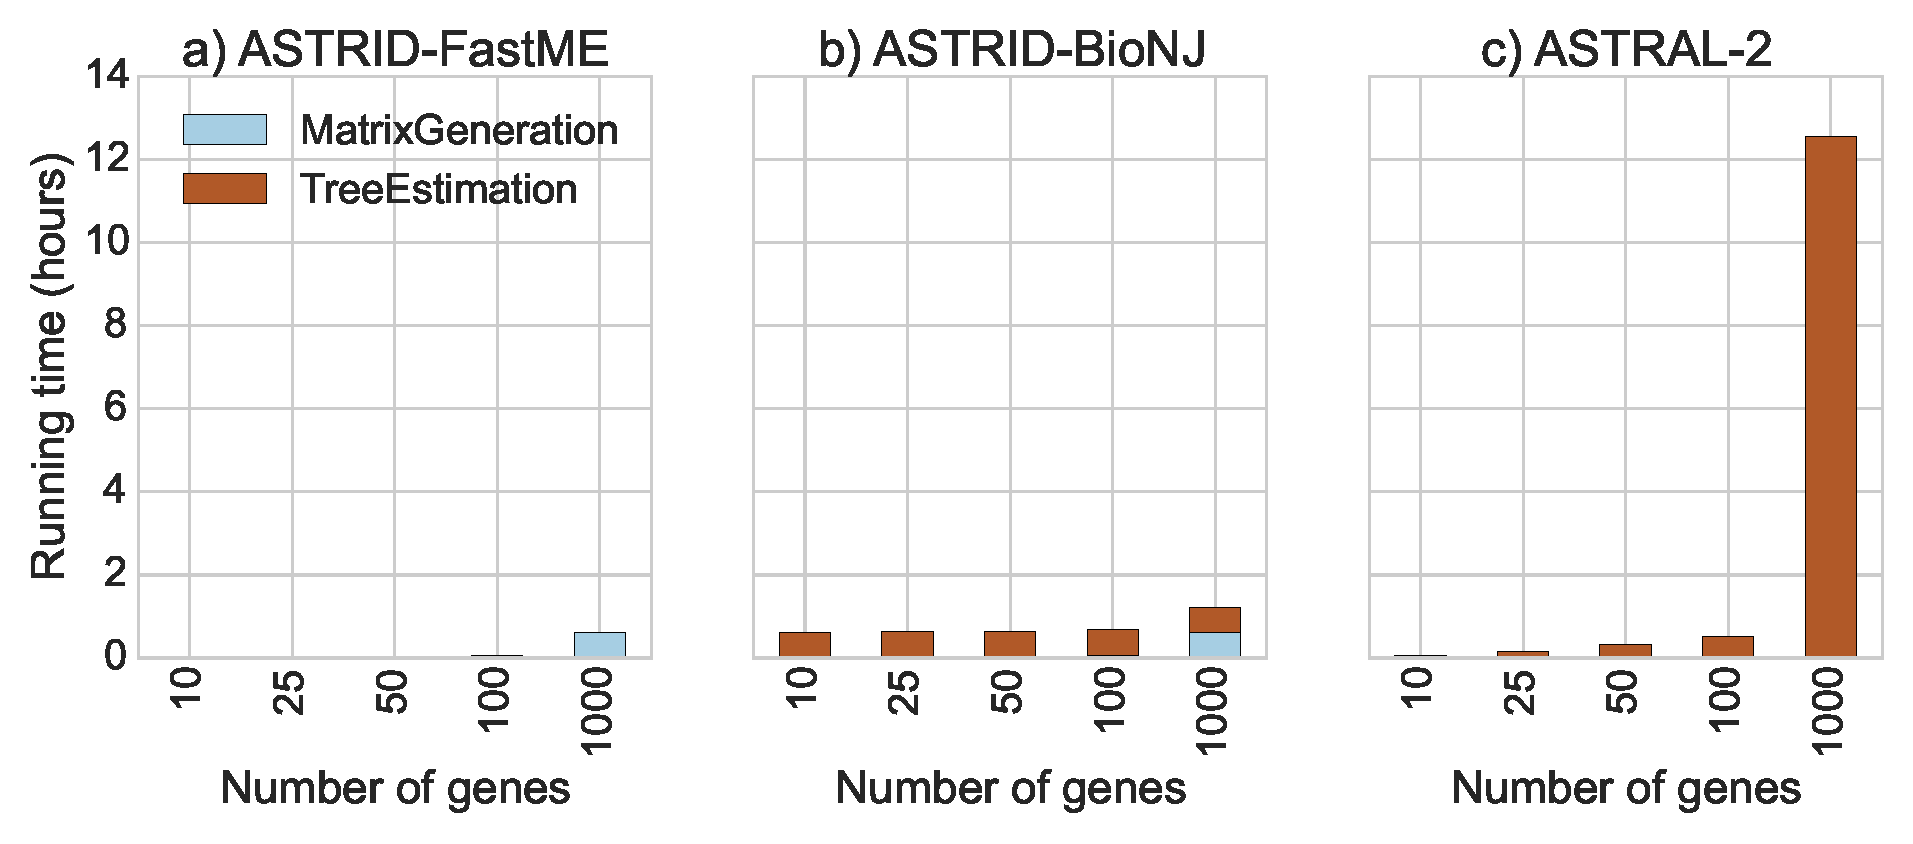
\includegraphics[width=12cm]{astrid-figs/1000-timing.eps}
  \caption[Running time 
on the ASTRAL-2 
    simulated datasets with 1000 taxa]{\textbf{Running time 
on the ASTRAL-2 
    simulated datasets with 1000 taxa (MC11), varying number of
    genes.} 
We show results for the each of the ASTRID steps -- matrix generation 
and tree estimation. We compare ASTRID used with two
ways of computing the trees: FastME and BioNJ*.
Experiments were run on a single core of a 2.7 GHz Intel Xeon processor. 
}
  \label{astrid::fig:1000-timing}
\end{figure}


\begin{figure}
  \centering
  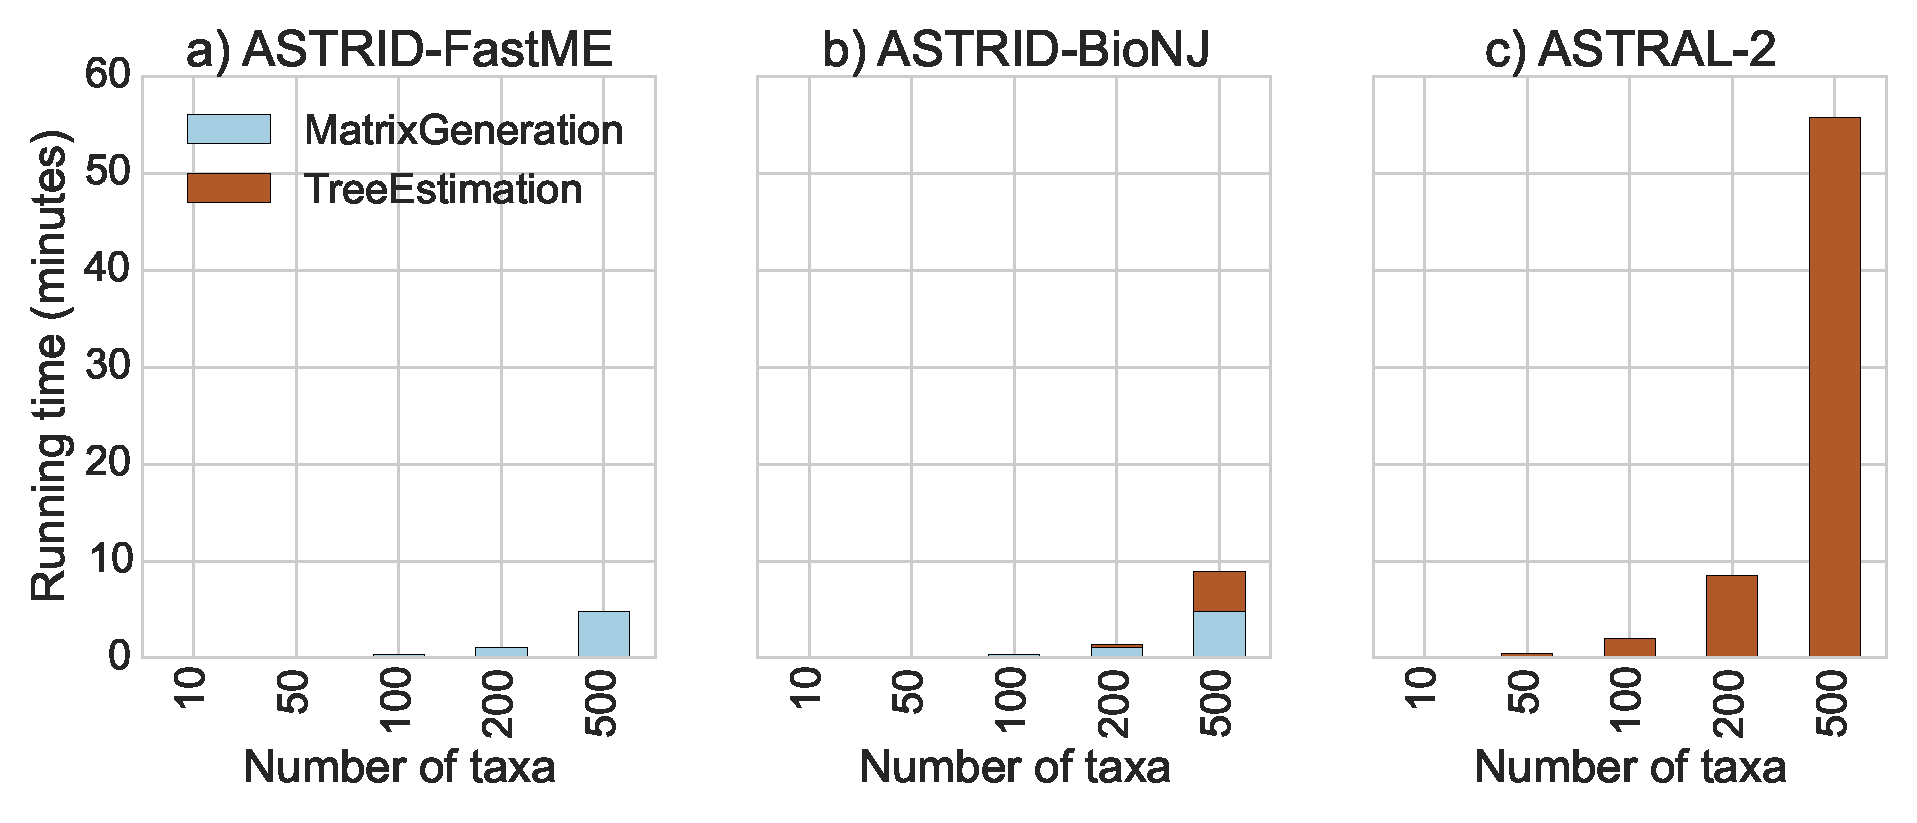
\includegraphics[width=12cm]{astrid-figs/astral-timing.eps}
  \caption[Running time of two ASTRID methods on the ASTRAL-2 
    simulated dataset, varying number of
    taxa.]{\textbf{Running time of two ASTRID methods on the ASTRAL-2 
    simulated dataset with 500 genes, varying number of
    taxa.} We show results on a single
replicate of model conditions MC2 and 7-10 from
the ASTRAL-2 collection. Experiments were run on a single core of a 2.7 GHz Intel
    Xeon processor.}
  \label{astrid::fig:astral-timing}
\end{figure}

\section{Discussion}

A few trends are apparent upon examining the data as a whole. ASTRAL-2 
and ASTRID had, for the most part, very similar levels of accuracy,
while MP-EST was consistently less accurate.  However, there were cases 
where ASTRID and ASTRAL-2 have small but detectably different levels of
accuracy.
One intriguing trend in the data is the improvement of
ASTRAL-2 over ASTRID on high ILS datasets; see Figures~\ref{astrid::fig:mammalian-ils},
\ref{astrid::fig:astral2-ils}, \ref{astrid::fig:15taxon}, and \ref{astrid::fig:10-taxon}. 
In particular, Figures \ref{astrid::fig:mammalian-ils} and \ref{astrid::fig:astral2-ils} suggest
that increases in ILS should favor ASTRAL-2 over ASTRID. Yet, 
 ASTRID is consistently 
at least as accurate as ASTRAL-2 on the avian datasets, which
have moderate to very high levels of ILS (Fig.~\ref{astrid::fig:avian-ils}).
Thus, ILS level might have an impact on the relative accuracy of the
two methods, but it is not a determining favor.
Similarly, neither method
dominates the other based on the number of
taxa, number of genes, or amount of gene tree estimation error.
Thus, it is very difficult to characterize the conditions under which each method is
likely to have an advantage over the other.
However, even for
the cases where there are differences in accuracy, in general the differences
are fairly small. Thus, the main difference between the two methods 
is computational efficiency, where ASTRID is clearly faster. ASTRID
has the biggest running time advantage over ASTRAL-2 for large numbers
of gene trees, since ASTRID scales linearly in the number of genes
while ASTRAL scales super-linearly. This makes ASTRID an especially
good method for genome-scale datasets that have a large number of
genes.
%Pranjal


\section{Conclusion}

ASTRID is a fast and highly accurate method for species tree
estimation that is robust to high levels of ILS, and provably
statistically consistent under the multi-species coalescent model.
Like ASTRAL-2, 
 ASTRID can analyze datasets with unrooted gene trees, an
advantage that the two methods have over many other methods (e.g.,
MP-EST) that can only be run on rooted gene trees.  
ASTRID (like NJst) runs in time that is polynomial in the number of gene
trees and species, but ASTRAL-2 
 and other leading coalescent-based
methods do not have this guarantee.  Thus, ASTRID has many desirable
theoretical properties compared to existing methods.

From an empirical viewpoint, ASTRID is also extremely fast and can
analyze very large datasets in minutes, where other methods either
cannot run or take hours.  In particular, ASTRID is much faster than
ASTRAL-2, 
 especially on datasets with many genes and large numbers of
species.  ASTRID also produces more accurate trees than MP-EST and
NJst, and is competitive with ASTRAL-2 
 in terms of accuracy.

However, even better (more accurate) results might be obtained through
more extensive modifications to the ASTRID algorithm design. In
particular, the accuracy of the tree depends on the particular
distance-based method that is used. 
New distance-based phylogeny estimation methods, such as
the absolute fast converging methods 
\cite{afc,roch-science}, might provide 
improved accuracy for very large datasets with many thousands of 
species.
Another important direction is developing additional methods 
for estimating species trees from distance matrices that have good
accuracy when the distance matrix has missing data. As we saw here,
FastME produced more accurate trees than the PhyD* methods, but it
could only be applied to distance matrices without any missing data.
An extension of FastME to enable it to handle incomplete distance matrices
would also be of great interest.


This study can be expanded in several directions.
Future work should more carefully investigate the conditions 
under which ASTRID is more reliable than ASTRAL-2, and explore
performance on more biological datasets. 
This study also only investigated relatively
long sequences; a subsequent study should investigate 
the relative and absolute accuracy of ASTRID and other methods
on very short sequences, since
recombination-free loci can be very short \cite{GatesyMPE2014}.
In addition, this study only examined datasets with a single
individual per species, yet ASTRID 
(like NJst)
can be run on datasets with multiple individuals;
future work should  
evaluate the absolute and relative accuracy of ASTRID and other methods
on such data.
This study showed that  ASTRID performed well in terms of species tree topology estimation, but 
we did not explore its accuracy with respect to the estimation of 
coalescent branch lengths; future work will need to explore how well
ASTRID estimates
these numeric parameters.
Finally, it may well be that ASTRID will be most useful as
a starting tree for use within more 
computationally intensive analyses, including
Bayesian MCMC analyses (e.g., *BEAST) or
maximum likelihood analyses.
